\documentclass[a4paper,12pt]{report}
% \usepackage[english]{babel}

% Set page size and margins
\usepackage[a4paper,top=2cm,bottom=2cm,left=2.5cm,right=2.5cm,marginparwidth=1.75cm]{geometry}

% Useful packages
\usepackage{amsmath,amssymb}
\usepackage{graphicx}
\usepackage{algorithm}
\usepackage{algpseudocode}
\usepackage{hyperref}
\usepackage{booktabs}
\usepackage{lscape}
\usepackage{longtable}
\usepackage{multicol}
\hypersetup{
    colorlinks=false,
    linkcolor=blue,
    filecolor=magenta,      
    urlcolor=cyan,
    pdftitle={World Trade Thesis},
    pdfpagemode=FullScreen,
    }
    
% % \urlstyle{same}
\usepackage[sorting=none,style=numeric]{biblatex}
% \usepackage{fontspec}
% \defaultfontfeatures{Mapping=tex-text}
% \setmainfont{Verdana}
% \renewcommand{\familydefault}{\sfdefault}

% \usepackage{csvsimple}

% \begin{filecontents*}{cpa21_l2.csv}
"Order","Level","Code","Parent","Description","This_item_includes","This_item_also_includes","Rulings","This_item_excludes"
"1208793","2","01","A","Products of agriculture, hunting and related services",,,,
"1209066","2","02","A","Products of forestry, logging and related services",,,,"This division excludes:
- 	sawing and planing of wood, see appropriate group of division 16"
"1209099","2","03","A","Fish and other fishing products; aquaculture products; support services to fishing",,,,"This division excludes:
- services auxiliary to sport and recreational fishing, see 93.19.13"
"1209137","2","05","B","Coal and lignite",,,,"This division excludes:
- 	test drillings services for coal and services connected with coal extraction, see 09.90.11
- coke oven products, see 19.10
- coal briquettes, see 19.20.1
- site preparation for the extraction of coal, see 43.12.11"
"1209146","2","06","B","Crude petroleum and natural gas",,,,"This division excludes:
- 	probing, test drillings and exploration works in connection with petroleum and gas extraction, see 09.10.1
- services related to operation of oil and gas fields, on a fee or contract basis, see 09.10.1
- 	refined petroleum products, see 19.20
- transport via pipeline of crude or refined petroleum and petroleum products, see 49.50.11
- transport via pipeline of natural gas, see 49.50.12
- 	geophysical surveys and cartographic activities, see 71.12.3"
"1209157","2","07","B","Metal ores",,,,"This division excludes:
- roasted iron pyrites, see 20.13.67
- aluminium hydroxide, see 20.13.25 
- aluminium oxide, see 24.42.12"
"1209174","2","08","B","Other mining and quarrying products",,,,"This division excludes:
- processing of extracted raw materials (excl. crushing, grinding, cutting, cleaning, drying, sorting and mixing), see appropriate parts of section C"
"1209213","2","09","B","Mining support services",,,,"This division excludes: 
- specialised repair services of mining machinery, see 33.12.24
- services related to liquefaction and regasification of natural gas for transportation off the mine site, see 52.21"
"1209226","2","10","C","Food products","This division includes: 
- a variety of products that are the effect of farming, forestry, hunting and fishing, such as meat, fish, fruits and vegetables, fats and oils, dairy products, grain mill products, animal feeds and other food products intended for humans or animals
- semi-finished products that are not directly food products 
- by-products of different value in use (e.g. the hides, oil-cake from the production of vegetable oils)
- treatment of slaughterhouse waste/waste seized at slaughterhouses/for the production of animal feed",,,"This division excludes:
- processing of food waste and waste from the production of beverages into secondary raw materials, see 38.3, and their removal, see 38.21
- food preparation for immediate consumption (e.g. in restaurants), see 56.10.1
- services related to the packaging of meat carried out on a fee or contract basis, see 82.92.10"
"1209551","2","11","C","Beverages",,,,"This division excludes:
- fruit and vegetable juices, see 10.32.1
- non-alcoholic beverages based on milk, see 10.51.5
- coffee, tea and maté (Paraguay tea), see 10.83.1"
"1209594","2","12","C","Tobacco products",,,,"This division excludes:
- tobacco growing, see 01.15.10
- drying tobacco leaves, see 01.63.10"
"1209605","2","13","C","Textiles",,,,
"1209740","2","14","C","Wearing apparel",,,,
"1209831","2","15","C","Leather and related products",,,,
"1209877","2","16","C","Wood and of products of wood and cork, except furniture; articles of straw and plaiting materials",,,,"This division excludes:
- furniture, see division 31"
"1209953","2","17","C","Paper and paper products",,,,
"1210037","2","18","C","Printing and reproduction services of recorded media",,,,
"1210069","2","19","C","Coke and refined petroleum products",,,,
"1210105","2","20","C","Chemicals and chemical products",,,,
"1210373","2","21","C","Basic pharmaceutical products and pharmaceutical preparations",,,,
"1210407","2","22","C","Rubber and plastic products",,,,
"1210489","2","23","C","Other non-metallic mineral products",,,,
"1210662","2","24","C","Basic metals",,,,
"1210859","2","25","C","Fabricated metal products, except machinery and equipment",,,,"This division excludes:
- machinery and equipment, see division 28"
"1211010","2","26","C","Computer, electronic and optical products",,,,
"1211193","2","27","C","Electrical equipment",,,,
"1211353","2","28","C","Machinery and equipment n.e.c.",,,,
"1211690","2","29","C","Motor vehicles, trailers and semi-trailers",,,,
"1211754","2","30","C","Other transport equipment",,,,
"1211859","2","31","C","Furniture",,,,
"1211899","2","32","C","Other manufactured goods",,,,
"1212019","2","33","C","Repair and installation services of machinery and equipment",,,,
"1212100","2","35","D","Electricity, gas, steam and air conditioning",,,,
"1212133","2","36","E","Natural water; water treatment and supply services",,,,
"1212143","2","37","E","Sewerage services; sewage sludge",,,,
"1212151","2","38","E","Waste collection, treatment and disposal services; materials recovery services",,,,
"1212241","2","39","E","Remediation services and other waste management services",,,,
"1212254","2","41","F","Buildings and building construction works",,,,
"1212287","2","42","F","Constructions and construction works for civil engineering",,"This division also includes:
- development of civil engineering projects.",,"This division excludes:
- development of building projects, see 41.00"
"1212339","2","43","F","Specialised construction works",,,,
"1212411","2","45","G","Wholesale and retail trade and repair services of motor vehicles and motorcycles",,,,
"1212481","2","46","G","Wholesale trade services, except of motor vehicles and motorcycles",,,,"This division excludes:
- wholesale trade services of motor vehicles and motorcycles, see division 45"
"1212721","2","47","G","Retail trade services, except of motor vehicles and motorcycles",,,,"This division excludes:
- retail trade services of motor vehicles and motorcycles, see division 45"
"1212800","2","49","H","Land transport services and transport services via pipelines",,,,
"1212865","2","50","H","Water transport services",,,,
"1212906","2","51","H","Air transport services",,,,
"1212930","2","52","H","Warehousing and support services for transportation",,,,
"1212981","2","53","H","Postal and courier services",,,,
"1212997","2","55","I","Accommodation services",,,,
"1213020","2","56","I","Food and beverage serving services",,,,
"1213044","2","58","J","Publishing services",,,,
"1213134","2","59","J","Motion picture, video and television programme production services, sound recording and music publishing",,,,
"1213184","2","60","J","Programming and broadcasting services",,,,
"1213204","2","61","J","Telecommunications services",,,,
"1213251","2","62","J","Computer programming, consultancy and related services",,,,
"1213276","2","63","J","Information services",,,,
"1213302","2","64","K","Financial services, except insurance and pension funding",,,,"This division excludes:
- insurance, reinsurance and pension funding services, see division 65"
"1213346","2","65","K","Insurance, reinsurance and pension funding services, except compulsory social security",,,,"This division excludes:
- compulsory social security services, see division 84"
"1213406","2","66","K","Services auxiliary to financial services and insurance services",,,,
"1213449","2","68","L","Real estate services",,,,
"1213478","2","69","M","Legal and accounting services",,,,
"1213506","2","70","M","Services of head offices; management consulting services",,,,
"1213528","2","71","M","Architectural and engineering services; technical testing and analysis services",,,,
"1213572","2","72","M","Scientific research and development services",,,,"This division excludes:
- market research services, see 73.20.11"
"1213648","2","73","M","Advertising and market research services",,,,
"1213675","2","74","M","Other professional, scientific and technical services",,,,
"1213716","2","75","M","Veterinary services",,,,
"1213724","2","77","N","Rental and leasing services",,,,"This division excludes:
- financial leasing services, see 64.91.10"
"1213781","2","78","N","Employment services",,,,
"1213807","2","79","N","Travel agency, tour operator and other reservation services and related services",,,,
"1213835","2","80","N","Security and investigation services",,,,
"1213850","2","81","N","Services to buildings and landscape",,,,
"1213876","2","82","N","Office administrative, office support and other business support services",,,,
"1213909","2","84","O","Public administration and defence services; compulsory social security services",,,,
"1213967","2","85","P","Education services",,,,
"1214038","2","86","Q","Human health services",,,,
"1214072","2","87","Q","Residential care services",,,,
"1214094","2","88","Q","Social work services without accommodation",,,,
"1214116","2","90","R","Creative, arts and entertainment services",,,,
"1214134","2","91","R","Library, archive, museum and other cultural services",,,,
"1214152","2","92","R","Gambling and betting services",,,,
"1214164","2","93","R","Sporting services and amusement and recreation services",,,,
"1214194","2","94","S","Services furnished by membership organisations",,,,
"1214225","2","95","S","Repair services of computers and personal and household goods",,,,
"1214257","2","96","S","Other personal services",,,,
"1214290","2","97","T","Services of households as employers of domestic personnel",,,,
"1214299","2","98","T","Undifferentiated goods and services produced by private households for own use",,,,
"1214309","2","99","U","Services provided by extraterritorial organisations and bodies",,,,

\end{filecontents*}


% Custom operators
%\DeclareMathOperator{\E}{\mathbb{E}}
%\DeclareMathOperator{\cal}[1]{\mathcal{#1}}
%\DeclareMathOperator{\fk}[1]{\mathfrak{#1}}
%\DeclareMathOperator{\bf}[1]{\mathbf{#1}}
%\DeclareMathOperator{\kl}[2]{KL \left( #1\,||\,#2 \right)}
%\newtheorem{definition}{Definition}[section]

\title{World Trade Thesis}
\author{Pietro Dominietto}
\date{October 2022}

\bibliography{references}


\begin{document}
\maketitle

% \begin{abstract}
% Abstract
% \end{abstract}


\tableofcontents

% \pagebreak

% Introduction chapter
\chapter{Introduction chapter}

% ISTAT used a publicly available dataset (COMEXT, by Eurostat) which contains historical data about world imports and exports of goods since 2010, to gather insights and in the end produce a web tool to provide useful statistics and a graph visualization of the commerce network. 
The core idea of the research I've conducted is to construct a dataset about world import and exports of goods among world countries, to represent it as a directed graph and to produce insights about world trade using mathematical and statistical tools.
The inspiration for this work comes from the research internship I did with ISTAT (Italian National Institute of Statistics) and their previous research named \textit{Cosmopolitics}. % CITATION 
They used a publicly available dataset named COMEXT by \textcite{eurostat2022comext}, which contains, among other things, historical data about world imports and exports reported by EU countries, from 1988 until 2022. The project that they developed consisted in a web tool to provide useful statistics and a graph visualization of the European commerce network.\footnote{Tool online at  \href{https://cosmo.statlab.it/}{cosmo.statlab.it} Code available here \url{https://github.com/istat-methodology/cosmopolitics}}


\section{Research questions}

Now they are wondering what else could they exploit these data for:
\begin{itemize}
    \item Can we use the graph representation of the good exchanges to understand the commerce network and look at useful statistics of the graph, and how they relate to real world effects?
    \item[OLD] \textit{Starting from the graph representation of the commerce data, is it possible to train ML and NN methods (like GraphNN and Bayes Nets) to make predictions, evaluate scenarios and draw inferences on them?}
    \item Can we be able to build a model capable of learning how did commerce evolve through time and given the model be able to observe what changes happen in the system when we add, remove or modify a node or an edge?
    \item In fact, their research questions for my project are about using these data and the graphs generated to investigate whether it’s possible to apply ML and NN methods (like Bayesian Nets or GraphNNs) to draw inferences about the graphs and evaluate scenarios or compute forecasts.
\end{itemize}
% Boh
\chapter{World trade and literature review}

% \section{What is this work about for dummies}
% Key idea: this thesis will be read by people that don't really know a nut about statistics and data analysis. 
% So, what is this work about? 
% The core points are the following:
% \begin{itemize}
%     \item Analysis of the data is conducting us to observe the same results one could easily spot in real life scenarios (did I understand correctly?)
%     \item Some new technique you used (if any)
% \end{itemize}
% \section{What is significant and unique about this study}
% why is this important and / or interesting? Why should this thesis be read?
% \section{SOTA}
% self explanatory
% \section{Data analysis for dummies (?)}
% Brief explanation of what is data analysis, core methods? I dunno

% Data and Graphs chapter
%% TODO: in the chapter, better explain "the purpose of the analysis" once ch 2 is done

\chapter{From the data to the graphs}
% mao bacini tantiii siiiiii
The goal of this chapter is to illustrate the data collection process and the procedures for data cleaning and integration that were undertaken. This part of the research is fundamental, since the validity of each following step depends on the reliability of the data that one is working with. In particular, the accuracy of any kind of insights and conclusions that one may draw about the networks and the scenarios that are observed is deeply rooted in the data gathering process.
Finding a unique and consistent data source for the purpose of this analysis was quite demanding, and in fact in the end I needed to combine information coming from multiple datasets. The following section will start by illustrating the multiple sources I have used including details and information about them, then I will move on into explaining the sequence of step I applied on the data to construct, in the end, the graphs and networks that are the base of my analysis.

\section{Data Sources}

The data needed for constructing the networks and performing the analysis come from multiple sources, and there are two main reasons for this: one is because the original dataset was incomplete about the world's trade network, and the second one is because, in order to be able to compare exchanges of different countries, I needed to have external exogenous variables that would give me additional information about the countries. In particular, the data sources that I employed are:
\begin{itemize}
    \item European Statistical Office (Eurostat) \cite{eurostat2022comext}, for the COMEXT dataset on European trade;
    \item World Trade Organization (WTO) \cite{wto2022stats}, for their dataset on global trade including non-EU countries;
    \item United Nations (UN) \cite{un2022population}, for the estimates of population that I used as exogenous variable;
    \item European Central Bank (ECB) \cite{ecb2021usdeur}, for the USD-EUR historical exchange rates that I needed to combine the datasets.
\end{itemize}

\subsection{COMEXT}

The starting dataset of my research is named COMEXT, and is published and maintained by Eurostat \cite{eurostat2022comext}. COMEXT is a statistical database for detailed statistics on international trade in goods\footnote{The definition of \textit{goods} provided by Eurostat is "\textit{all movable property including electricity}".}. It serves as an important indicator of the performance of the European Union (EU) economy, because it focuses on the size and the evolution of imports and exports of countries. It provides access not only to both recent and historical data of the EU and its individual Member States, but also to statistics of a significant number of non-EU countries. The information contained in it is based on data provided by the statistical agencies of the EU member states and trading partners.
Data are organized in tables, one for each year (or for each month) and each table contains information about the country that declared the transaction, the partner country, the product that was exchanged according to multiple international standard classifications (or nomenclatures), the value in euros of the exchange and its quantity in kilograms.
Let us now have a look at an extraction from this dataset, as you can see in Table \ref{tab:comextexample}.
The data available follow the shown format. Each row corresponds to a transaction, an exchange of a certain good between two countries in a given period. The information available about each transaction is summarized here:
\begin{itemize}
    \item \textit{DECLARANT} and \textit{DECLARANT ISO}: code and ISO\footnote{ISO stands for International Standardization Organization, which harmonizes codes and abbreviations across the world (\url{www.iso.org}). The conversion is displayed in Appendix Table \ref{tab:iso2}.} name of the country that declared the trade;
    \item \textit{PARTNER} and \textit{PARTNER ISO}: code and ISO name of the country with which the declarant traded;
    \item \textit{TRADE TYPE}: indicates whether the exchange was among two EU countries (I) or one was extra-EU (E);
    \item all the \textit{PRODUCT} columns: they are used to classify the good that was exchanged, according to different nomenclatures and standards;
    \item \textit{FLOW}: indicates whether the exchange was reported as an import (1) by the declarant or as an export (2);
    \item \textit{PERIOD}: indicates the time period of the exchange, in the format \texttt{yyyymm}\footnote{If it refers to a whole year then the format is \texttt{yyyy52}.};
    \item \textit{VALUE IN EUROS}: indicates the monetary value of the exchange between countries of that product;
    \item \textit{QUANTITY IN KG}: indicated the weight in kilograms of the exchange between countries of that product.
\end{itemize}
\begin{landscape}
\begin{table}
    \centering
    \resizebox{1.6\textheight}{!}{
\begin{tabular}{rrrrrrrrrrrrrrrrrrrr}
% \begin{tabular}{p{2.5cm}p{2.5cm}p{2cm}p{2cm}p{2cm}p{2cm}p{2cm}p{2cm}p{2cm}p{2cm}p{2cm}p{2cm}p{2cm}p{2cm}p{2cm}p{2cm}p{2cm}}
 \toprule
 DECLARANT & DECLARANT ISO & PARTNER & PARTNER ISO & TRADE TYPE & PRODUCT NC & PRODUCT SITC & PRODUCT cpa2002 & PRODUCT cpa2008 & PRODUCT CPA2 1 & PRODUCT BEC & PRODUCT SECTION & FLOW & PERIOD & VALUE IN EUROS & QUANTITY IN KG \\ \midrule
 61 & CZ & 4 & DE & I & 83023000 & 69915 & 2863 & 2572 & 2572 & 530 & 15 & 2 & 200101 & 284650 & 137370 \\
 5 & IT & 604 & LB & E & 85011010 & 71610 & 3110 & 2711 & 2711 & 410 & 16 & 2 & 200101 & 42089 & 11200 \\
 7 & IE & 5 & IT & I & 20021010 & 05672 & 1533 & 1039 & 1039 & 122 & 04 & 1 & 200101 & 97333 & 207000 \\
 4 & DE & 52 & TR & E & 85363030 & 77253 & 3120 & 2712 & 2712 & 420 & 16 & 2 & 200101 & 124054 & 3200 \\
 1 & FR & 720 & CN & E & 84823000 & 74630 & 2914 & 2815 & 2815 & 420 & 16 & 2 & 200101 & 18294 & 1300 \\
 30 & SE & 64 & HU & E & 72193310 & 67553 & 2710 & 2410 & 2410 & 220 & 15 & 2 & 200101 & 36002 & 18000 \\
 7 & IE & 720 & CN & E & 82089000 & 69561 & 2862 & 2573 & 2573 & 420 & 15 & 1 & 200101 & 15039 & 400 \\
 60 & PL & 1 & FR & I & 70091000 & 66481 & 2612 & 2312 & 2312 & 220 & 13 & 1 & 200101 & 12724 & 845 \\
 46 & MT & 400 & US & E & 85442000 & 77312 & 3130 & 2732 & 2732 & 220 & 16 & 1 & 200101 & 47203 & 0 \\
 30 & SE & 53 & EE & E & 62064000 & 84270 & 1823 & 1414 & 1414 & 620 & 11 & 1 & 200101 & 18944 & 500 \\
 1 & FR & 528 & AR & E & 90261099 & 87431 & 3320 & 2651 & 2651 & 410 & 18 & 2 & 200101 & 30657 & 500 \\
 3 & NL & 38 & AT & I & 28257000 & 52269 & 2412 & 2012 & 2012 & 220 & 06 & 2 & 200101 & 125073 & 20400 \\
 55 & LT & 5 & IT & I & 55103000 & 65187 & 1710 & 1310 & 1310 & 220 & 11 & 1 & 200101 & 26906 & 4033 \\
 5 & IT & 9 & GR & I & 84669195 & 72819 & 2940 & 2849 & 2849 & 420 & 16 & 2 & 200101 & 90529 & 5600 \\
 1 & FR & 4 & DE & I & 70140000 & 66595 & 2615 & 2319 & 2319 & 220 & 13 & 1 & 200101 & 410786 & 33400 \\
 5 & IT & 472 & TT & E & 94018000 & 82118 & 3611 & 3100 & 3100 & 410 & 20 & 2 & 200101 & 39182 & 25800 \\
 11 & ES & 75 & RU & E & 44091011 & 24830 & 2010 & 1610 & 1610 & 220 & 09 & 2 & 200101 & 27916 & 3000 \\
 61 & CZ & 3 & NL & I & 84807190 & 74918 & 2956 & 2573 & 2573 & 410 & 16 & 1 & 200101 & 167767 & 545 \\
 30 & SE & 39 & CH & E & 84563011 & 73113 & 2940 & 2841 & 2841 & 410 & 16 & 1 & 200101 & 295905 & 8500 \\
 32 & FI & 10 & PT & I & 48109190 & 64177 & 2112 & 1712 & 1712 & 220 & 10 & 2 & 200101 & 12252 & 13200 \\
 53 & EE & 54 & LV & E & 48229000 & 64291 & 2125 & 1729 & 1729 & 220 & 10 & 2 & 200101 & 14994 & 18678 \\
 6 & GB & 720 & CN & E & 84615011 & 73177 & 2940 & 2841 & 2841 & 410 & 16 & 1 & 200101 & 20997 & 1900 \\
 5 & IT & 60 & PL & E & 85189000 & 76492 & 3230 & 2640 & 2640 & 420 & 16 & 2 & 200101 & 250280 & 73200 \\
 5 & IT & 400 & US & E & 97020000 & 89620 & 9231 & 9003 & 9003 & 610 & 21 & 2 & 200101 & 12861 & 500 \\
 6 & GB & 61 & CZ & E & 84148079 & 74319 & 2912 & 2813 & 2813 & 410 & 16 & 2 & 200101 & 37962 & 2900 \\
 91 & SI & 5 & IT & I & 82074030 & 69564 & 2862 & 2573 & 2573 & 420 & 15 & 1 & 200101 & 17573 & 227 \\
 38 & AT & 92 & HR & E & 21032000 & 09842 & 1587 & 1084 & 1084 & 122 & 04 & 2 & 200101 & 17346 & 20200 \\
 1 & FR & 5 & IT & I & 39173231 & 58140 & 2521 & 2221 & 2221 & 220 & 07 & 1 & 200101 & 86548 & 29200 \\
 4 & DE & 52 & TR & E & 39173231 & 58140 & 2521 & 2221 & 2221 & 220 & 07 & 2 & 200101 & 75198 & 14400 \\
 6 & GB & 628 & JO & E & 84189990 & 74149 & 2923 & 2825 & 2825 & 420 & 16 & 2 & 200101 & 16498 & 10000 \\
 11 & ES & 4 & DE & I & 28129000 & 52241 & 2413 & 2013 & 2013 & 220 & 06 & 1 & 200101 & 17184 & 1800 \\
 8 & DK & 400 & US & E & 28183000 & 52266 & 2413 & 2013 & 2013 & 220 & 06 & 1 & 200101 & 140360 & 100000 \\
 4 & DE & 3 & NL & I & 82022000 & 69551 & 2862 & 2573 & 2573 & 420 & 15 & 1 & 200101 & 91395 & 3800 \\
 4 & DE & 63 & SK & E & 60012100 & 65512 & 1760 & 1391 & 1391 & 220 & 11 & 2 & 200101 & 48420 & 4200 \\
 92 & HR & 5 & IT & I & 94019080 & 82119 & 3611 & 3100 & 3100 & 220 & 20 & 1 & 200101 & 23887 & 10559 \\
 6 & GB & 8 & DK & I & 42029291 & 83199 & 1920 & 1512 & 1512 & 620 & 08 & 1 & 200101 & 73806 & 3100 \\
 11 & ES & 5 & IT & I & 85153100 & 73735 & 2940 & 2790 & 2790 & 410 & 16 & 1 & 200101 & 578296 & 29500 \\
 3 & NL & 386 & MW & E & 09024000 & 07414 & 0113 & 0127 & 0127 & 112 & 02 & 1 & 200101 & 97484 & 65000 \\
 17 & BE & 732 & JP & E & 39032000 & 57291 & 2416 & 2016 & 2016 & 220 & 07 & 1 & 200101 & 25108 & 5400 \\
 11 & ES & 3 & NL & I & 08103030 & 05794 & 0113 & 0125 & 0125 & 112 & 02 & 1 & 200101 & 16854 & 6200 \\
 1 & FR & 3 & NL & I & 72042900 & 28229 & 2710 & 3811 & 3811 & 210 & 15 & 2 & 200101 & 59015 & 258300 \\
 4 & DE & 979 & QZ & E & 29211930 & 51451 & 2414 & 2014 & 2014 & 220 & 06 & 2 & 200101 & 381600 & 372300 \\
 6 & GB & 17 & BE & I & 30021091 & 54163 & 2442 & 2120 & 2120 & 220 & 06 & 1 & 200101 & 4166599 & 1500 \\
 7 & IE & 6 & GB & I & 85421360 & 77641 & 3210 & 2611 & 2611 & 420 & 16 & 2 & 200101 & 438109 & 0 \\
 1 & FR & 640 & BH & E & 84431990 & 72659 & 2956 & 2899 & 2899 & 410 & 16 & 1 & 200101 & 41257 & 300 \\
 11 & ES & 3 & NL & I & 72193410 & 67554 & 2710 & 2410 & 2410 & 220 & 15 & 1 & 200101 & 118787 & 59300 \\
 7 & IE & 220 & EG & E & 84733090 & 75997 & 3002 & 2620 & 2620 & 420 & 16 & 2 & 200101 & 184452 & 1500 \\
 3 & NL & 388 & ZA & E & 90261051 & 87431 & 3320 & 2651 & 2651 & 410 & 18 & 2 & 200101 & 48644 & 900 \\
 1 & FR & 30 & SE & I & 84733010 & 75997 & 3002 & 2620 & 2620 & 420 & 16 & 2 & 200101 & 1138762 & 3800 \\
 60 & PL & 94 & YU & E & 16042090 & 03716 & 1520 & 1020 & 1020 & 122 & 04 & 2 & 200101 & 14171 & 9900 \\
 \bottomrule
\end{tabular}
}

    \caption{Random sample taken from the COMEXT dataset referring to imports and exports exchanged during January 2001.}
    \label{tab:comextexample}
\end{table}
\end{landscape}

\paragraph{Summary statistics}
Thanks to COMEXT data, we are able to conduct many types of analyses on commerce among countries. A first look at the data tells us that, by exploiting the variables that we have at disposal, we can observe if there are any trends in the EU economy as a whole, aggregating on all countries and products. This is shown in Figure \ref{fig:totaleu}. 

\begin{figure}
    \centering
    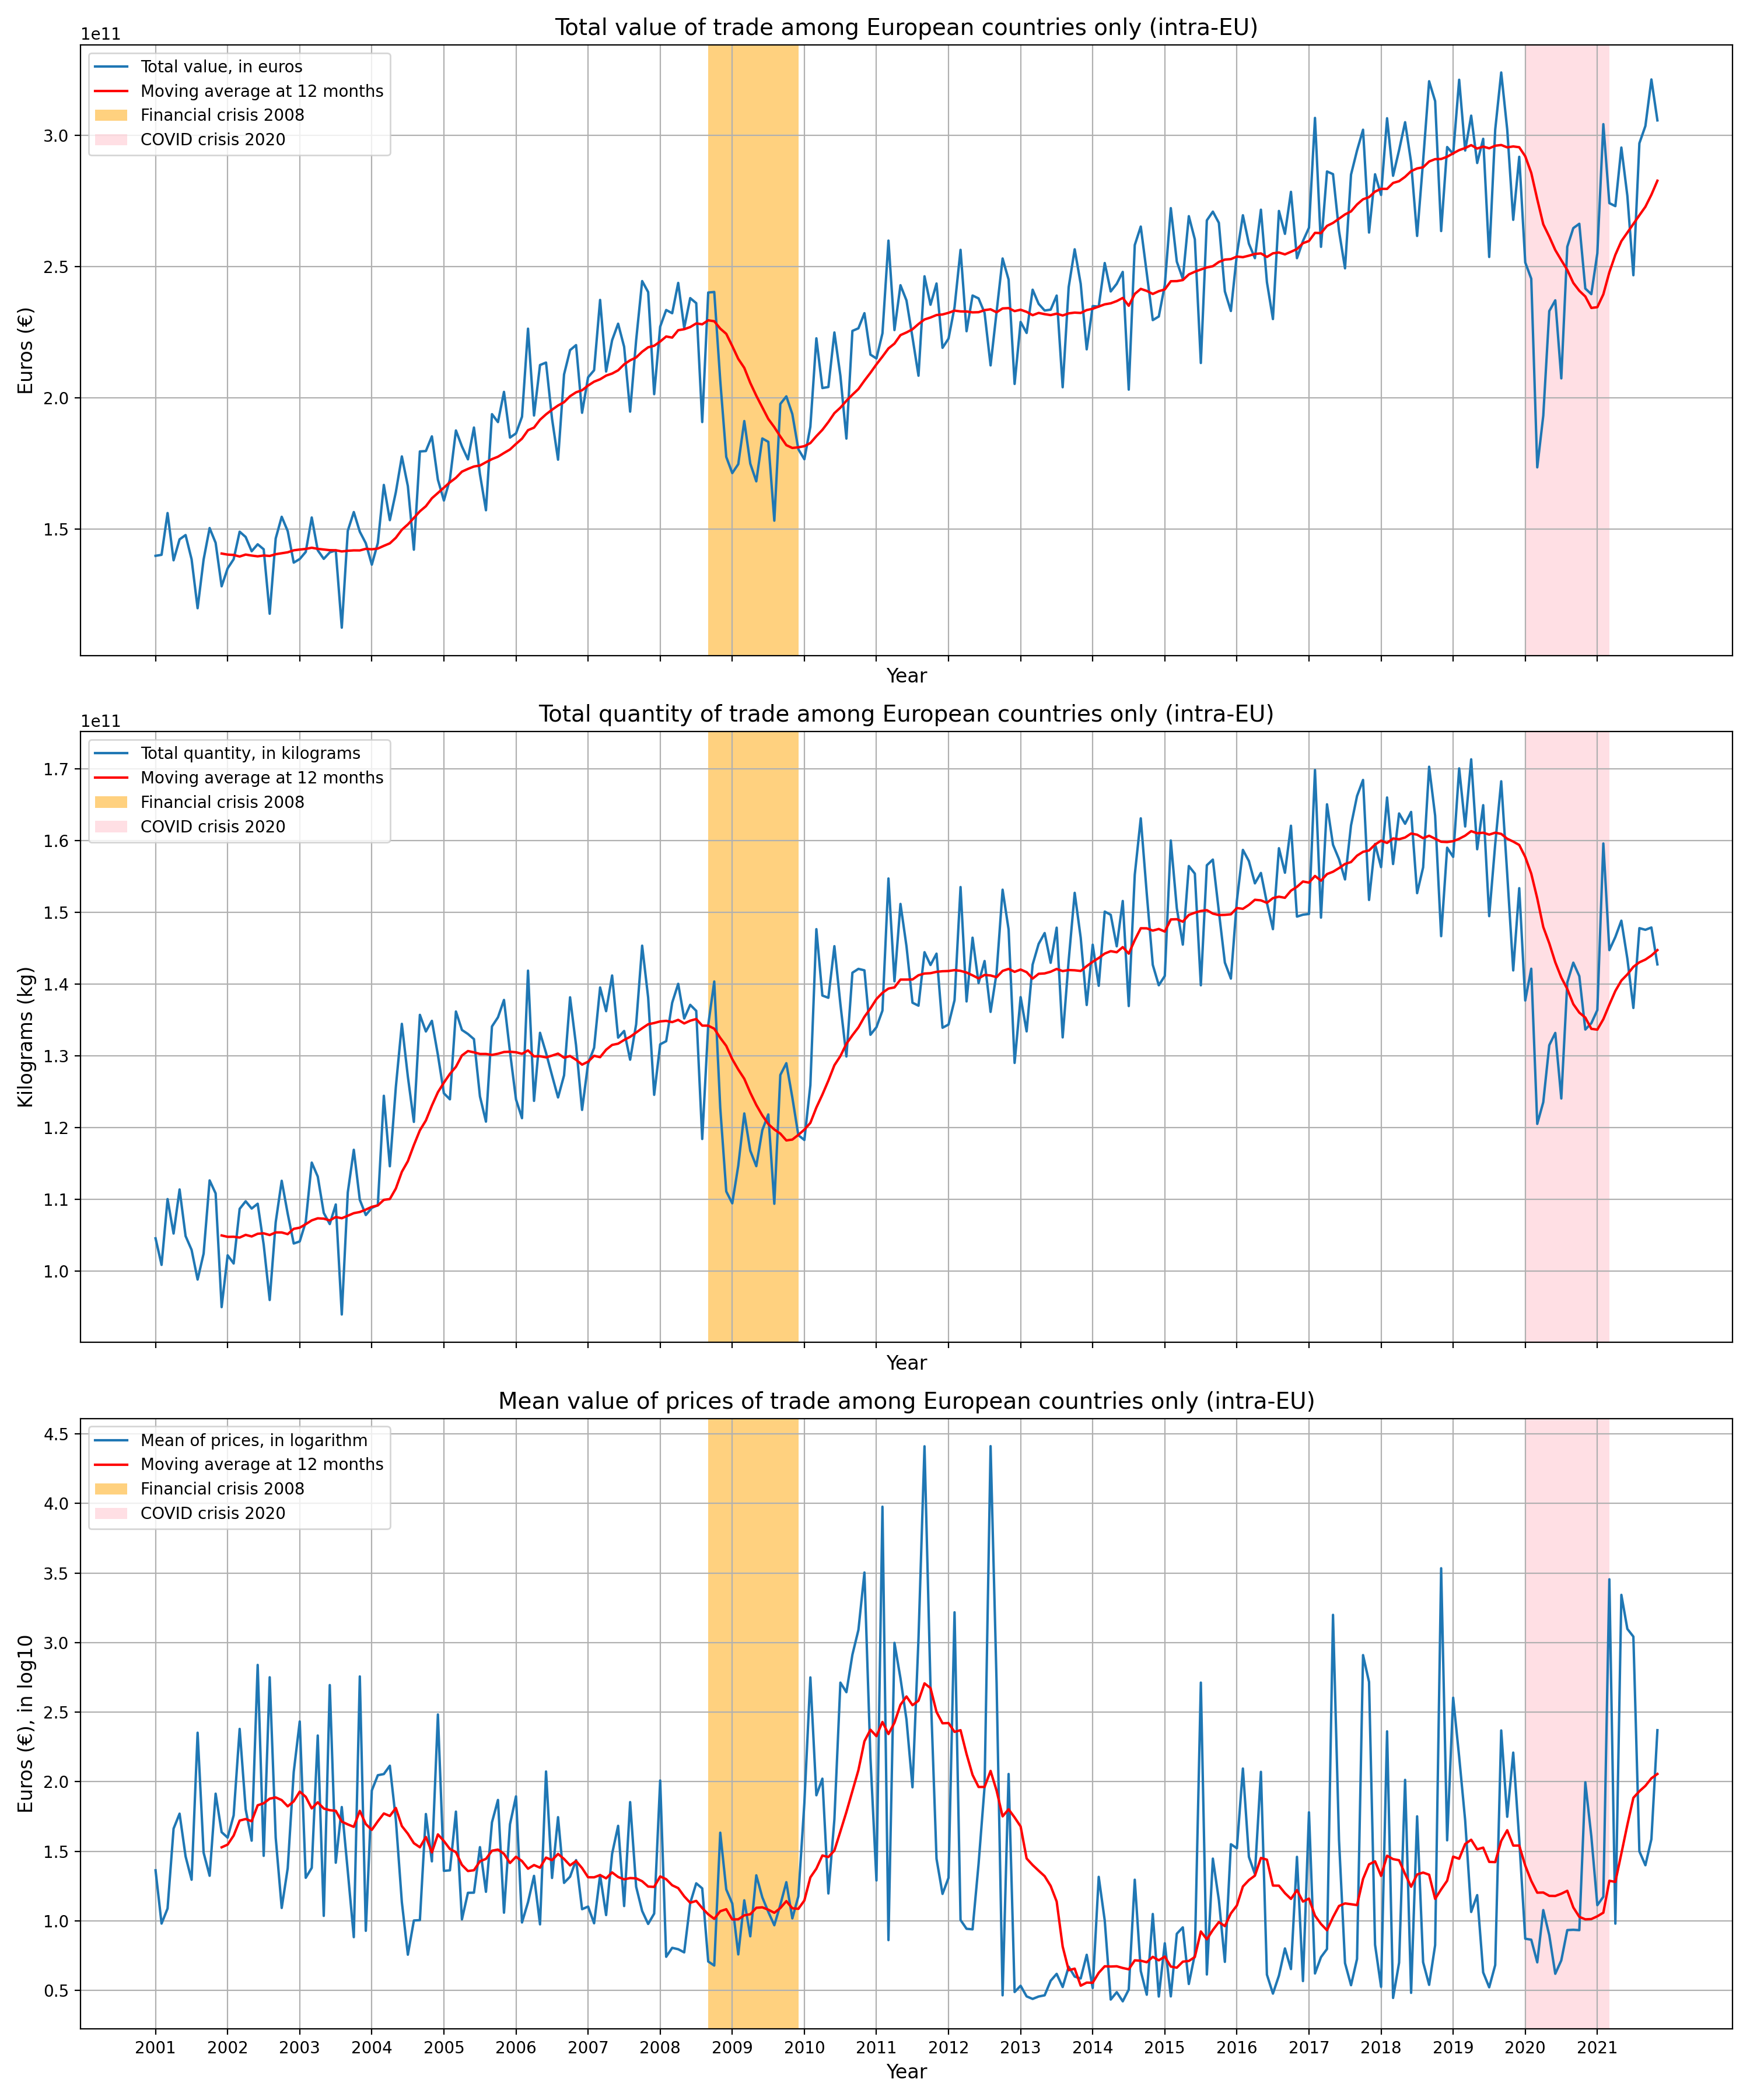
\includegraphics[width=\textwidth]{pics/TOTAL_VQP_INTRA.png}
    \caption[Long term trends of trade exchanges across EU member countries]{Long term trends of trade exchanges across EU member countries, by various indicators: (1) value (\texteuro), (2) quantity (Kg), (3) price (\texteuro/kg).}
    \label{fig:totaleu}
\end{figure}

In the first plot, we have on the horizontal axis time in years, while on the vertical axis we have monetary value expressed in euros. What is shown here is an aggregated sum of the total value of products exchanged by EU countries among themselves (intra-EU trade). This can be interpreted as an important indicator of the state of the whole economy, and in fact we can recognize in it two of the major economic events that happened in the last two decades: the 2008 financial crisis and the 2020 COVID-19 epidemic and related economic fallout. Since 2004 the growth of intra-EU trade was stable and sustained, up until the second semester of 2008, where we see a notable drop in total value, and a reprise only after the end of 2009. A similar effect can be seen at the beginning of 2020, where the lockdown due to the epidemic caused a sudden drop in the commerce of non-essential products, which almost brought the economy to a halt. Then production reprised in the second half of 2020, and we need to wait until 2021 for the values to reach pre-COVID levels.
If we look instead at the big picture, we see that overall intra-EU trade follows a positive trend that has basically doubled the value in 20 years. One has to wonder whether this increase in total money exchanged in commerce is due to an actual increase in production and circulation of goods, or is due just to inflation and higher prices of products. If we look at the second plot, we can observe the total quantity in kilograms of products exchanged in the EU economy. As before, we see a positive trend in the last 20 years, supporting our hypothesis that production has expanded. We also observe the same drops of trade exchanges following the two crises. Furthermore, what can be observed in both of the previous two plots is a yearly seasonality of these time series, where the values usually go up in the first trimester of the year, then they go down after mid-year, only to pick up again in the last part of the period. 
At last, in the third plot, we see the evolution of prices in the same time frame, obtained by dividing each exchange's value by its quantity. Note that the vertical axis is in log scale. Here we can see a different behavior than previously. While in the first eight years of the millennium prices of traded products have been going down, with less and less volatility year by year (which can also explain why demand and commerce of these goods has gone up), we can easily see that in the period following the 2008 crisis they went rapidly up again. This is a known and reasonable effect of those events, since, when dealing with scarcity and uncertainty, prices naturally rise, and with them also variability. It took more than three years after 2009 for these inflated prices to go down, and it can be easily seen that by the start of 2014 they were even lower than before 2008. Then they started slowly to grow, as we observe a  slight positive trend until 2020, with periodical cycles which last about a year. After 2021, which marked a first step out of the pandemic with the diffusion of COVID vaccines, we see the economy picking up again, and, as with the aftermath of crises, also prices and volatility increase.

%%esempio di tabella che viene da COMEXT -- altrimenti così son solo parole
%%Questo può essere quello che ti avevo segnato come capitolo 3 -- spiegazione etc etc 
%%Descrizione e visualizzazione del dataset - dati nulli, dati non comuni

\paragraph{COMEXT Data collection}
Historically, the main source of information about trade transactions between countries are customs authorities, which provide detailed information on exports and imports of goods with a geographical breakdown.
The COMEXT system was conceived and implemented in the early 90s,  following the adoption of the European Single Market in 1993, when customs formalities between Member States were removed. Since then, it has been continuously adapted and re-engineered to take into account technological evolution and new users' needs. The data gathered are based on two data collection systems:
\begin{itemize}
    \item data on trade in goods with non-EU countries are collected by customs authorities and are based on the records of trade transactions in customs declarations;
    \item data of intra-EU exchanges are directly collected from trade operators once a month.
\end{itemize}

The COMEXT dataset, however, presents a problem if one wants to use it to build an analysis on world trade. In fact, the only data contained in it are the ones reported by European countries, or even less than that, members of the European Union. Therefore, if we look at the whole network of commerce, we are missing some relevant information: the trade of extra-EU countries among themselves, since they have no obligation to communicate to Eurostat their records.
For this reason, and because I want to conduct a complete analysis and have a complete overview of the trade network, I needed to find another source of information, which I then integrated with COMEXT.

\subsection{WTO}
Similar to Eurostat, also the World Trade Organization (WTO) collects data about the global commerce of products among countries \cite{wto2022stats}. Data are periodically sent to the organization from member countries, hence the dataset contains information about all the major world countries.
Its structure is similar to COMEXT, but with a few differences: in fact, the data points are available with an annual periodicity instead of monthly as for the ones supplied by Eurostat. In Table \ref{tab:wtoexample} we can see a sample extracted from this dataset. As before, each row corresponds to the sum of exchanges between two countries in a given year, and for each import we have the following information:
\begin{itemize}
    \item \textit{Reporting Country}: the country that reported the value to WTO;
    \item \textit{Partner Country}: the country that exported the product to the reporting country;
    \item \textit{Product Code}: the code that identifies the category of the product exchanged, according to the Harmonized System (HS) nomenclature;
    \item \textit{Year}: indicating the year which the number refers to;
    \item \textit{Value}: the amount in US dollars that corresponds to the exchanged products' worth.
\end{itemize}

\begin{table}
    \centering
    \resizebox{1.0\textwidth}{!}{
\begin{tabular}{lllllr}
\toprule
 Reporting Economy Code & Partner Economy Code & Product Or Sector Code & Unit Code & Year & Value \\
\midrule
 356 & 826 & 970190 & USD & 2014 & 26972 \\
 268 & 840 & 961900 & USD & 2019 & 16323 \\
 716 & 840 & 970110 & USD & 2011 & 1613 \\
 800 & 840 & 960990 & USD & 2010 & 1126 \\
 344 & 826 & 960899 & USD & 2010 & 399676 \\
 634 & 784 & 961800 & USD & 2017 & 42030 \\
 716 & 800 & 970110 & USD & 2013 & 15 \\
 050 & 840 & 960839 & USD & 2008 & 424 \\
 410 & 840 & 970500 & USD & 2016 & 1929898 \\
 048 & 840 & 961210 & USD & 2004 & 45543 \\
 124 & 840 & 961511 & USD & 2009 & 684780 \\
 076 & 840 & 961210 & USD & 2002 & 2689590 \\
 410 & 764 & 970300 & USD & 2014 & 448973 \\
 800 & 840 & 970110 & USD & 2016 & 424 \\
 454 & 840 & 961610 & USD & 2006 & 326 \\
 376 & 840 & 960899 & USD & 2013 & 25000 \\
 840 & 862 & 960920 & USD & 2005 & 161269 \\
 600 & 840 & 960899 & USD & 2015 & 2542 \\
 756 & 784 & 970190 & USD & 2013 & 947 \\
 807 & 840 & 960910 & USD & 2001 & 100 \\
 458 & 840 & 961320 & USD & 2002 & 71548 \\
 834 & 792 & 960990 & USD & 2010 & 3 \\
 646 & 800 & 960899 & USD & 2018 & 17 \\
 352 & 764 & 961590 & USD & 2008 & 294 \\
 344 & 804 & 961800 & USD & 2013 & 50 \\
 222 & 840 & 962000 & USD & 2019 & 25475 \\
 124 & 764 & 961220 & USD & 2014 & 74935 \\
 702 & 764 & 961220 & USD & 2010 & 4077 \\
 268 & 784 & 960850 & USD & 2007 & 1200 \\
 356 & 826 & 961390 & USD & 2015 & 68 \\
 454 & 834 & 961700 & USD & 2013 & 3275 \\
 268 & 792 & 961390 & USD & 2005 & 1000 \\
 410 & 840 & 960850 & USD & 2007 & 4072 \\
 124 & 764 & 960910 & USD & 2009 & 507329 \\
 554 & 704 & 960910 & USD & 2012 & 219 \\
 156 & 704 & 970190 & USD & 2006 & 130 \\
 036 & 826 & 961320 & USD & 2006 & 4602 \\
 586 & 840 & 960860 & USD & 2004 & 6731 \\
 148 & 784 & 961590 & USD & 2012 & 3946 \\
 800 & 826 & 961511 & USD & 2016 & 6735 \\
 417 & 764 & 960910 & USD & 2017 & 1055 \\
 188 & 826 & 961000 & USD & 2005 & 10 \\
 792 & 840 & 961220 & USD & 2020 & 4682 \\
 616 & 792 & 961700 & USD & 2003 & 107 \\
 454 & 840 & 960990 & USD & 2008 & 208 \\
 764 & 704 & 960840 & USD & 2017 & 75 \\
 152 & 840 & 970400 & USD & 2001 & 1471 \\
 756 & 840 & 960891 & USD & 2020 & 3212 \\
 918 & 704 & 960899 & USD & 2001 & 3233 \\
 858 & 840 & 961610 & USD & 2008 & 3766 \\
\bottomrule
\end{tabular}
}
    \caption[Random sample taken from the WTO dataset]{Random sample taken from the WTO dataset, including codes of the HS nomenclature ranging from 960000 to 970000.}
    \label{tab:wtoexample}
\end{table}

Given the two available datasets, I had to find a way to combine them and to merge the variables of one with the other. Specifically, I needed to solve the following issues:
\begin{enumerate}
    \item The information about the European countries was repeated in both datasets, so it was necessary to choose which one to keep;
    \item The nomenclature for the products was different, so I used a conversion table and transformed one into the other;
    \item The monetary value of the exchange was in US dollars, so I converted it to Euros according to the exchange rate of that period.
\end{enumerate}

Hence, I proceeded as follows. For issue (1) I decided to keep the data from COMEXT and integrate them with WTO: this means that if we partition the countries in EU members and non-EU members, I get from COMEXT the data on intra-EU trade plus trade where one of the two countries is an EU member\footnote{More specifically, being an EU member for this purpose means that in that year the country has declared their numbers to Eurostat.}, while I get from WTO the rest of the trade data, that is, exchanges among two extra-EU countries.
Regarding issue (2), the solution was straightforward once I employed a conversion table, that allowed me to go from the HS classification to the CPA 2.1 nomenclature, as explained in Section \ref{sec:nomandusd}, while, for issue (3), in the same Section I'll show how the values were converted from US dollars to Euros, using a variable annual exchange rate.


\subsection{Nomenclatures and Currency}\label{sec:nomandusd}

In order to classify products into categories, many nomenclatures (or classifications) have been published by different organizations. Product classifications are designed to categorize products that have common characteristics. They provide the basis for collecting and calculating statistics on the production, distributive trade, consumption, international trade and transport of such products. The two datasets that I want to integrate, COMEXT and WTO, follow two different nomenclatures, created by two different institutions.
One of them is the Classification of Products by Activity (CPA), maintained by the European Commission and Eurostat.
According to Eurostat \cite{eurostat2022website}, "\textit{a statistical classification or nomenclature is an exhaustive and structured set of mutually exclusive and well-described categories, often presented in a hierarchy that is reflected by the numeric or alphabetical codes assigned to them, used to standardize concepts and compile statistical data}".
This procedure ensures that data is comparable between EU Member States, and for the purposes of this research, it enables us to put together reports of exchanges declared by different countries. While products in COMEXT are classified according to CPA, in the WTO dataset they follow the Harmonized Commodity Description and Coding System (HS), developed by the World Customs Organization (WCO) \cite{wco2022hs}. The system is used by more than 200 countries and economies as a basis for their Customs tariffs and for the collection of international trade statistics.\\
Although they have different categories and codes, these two nomenclatures have the same hierarchical structure: the classification starts with a super-category which is then broken down into smaller subcategories, adding more details to the description. This is highlighted by the digits or couple of digits of the numerical code that identifies the product. As an example, let us take the first row of Table \ref{tab:comextexample}, which is from COMEXT. The code in the column for CPA 2.1 is ``2572", and it is read in the following way:
\begin{itemize}
    \item The first two digits identify the broader category: in this case ``25" corresponds to \textit{Fabricated metal products, except machinery and equipment};
    \item The third digit identifies the first subcategory: ``257" corresponds to \textit{Cutlery, tools and general hardware};
    \item The fourth digit identifies the second subcategory: ``2572" corresponds to \textit{Locks and hinges}.
\end{itemize}
The analysis that will be conducted will focus only on the super-categories, that are identified by the first two digits of the code. The motivation behind this is that such classification is specific enough to be able to identify a relevant trade marked for these goods, but not too detailed so to fall into niche markets.
Therefore, before integrating the two data sources, what I needed to do was to convert the codes from the HS nomenclature in the WTO dataset into codes from the CPA 2.1, thanks to conversion tables provided by Eurostat\footnote{Available at \url{https://ec.europa.eu/eurostat/ramon/index.cfm} .}.

% PLOT WITH MAIN CATEGORIES
% TABLE WITH TWO DIGIT CPA CATEGORIES IN APPENDIX

% \paragraph{Currency exchange}\label{sec:usdeur}
The last issue to deal with when integrating the data is the change of currency, as I wanted to compare everything in euros. Since my purpose is to compare trade over time, I could not use a single value for the exchange rate. Hence, I used the dataset provided by the European Central Bank \cite{ecb2021usdeur}, which reports the weekly value of the exchange rates, as well as the annual value. The numbers I used are shown in Table \ref{tab:usdeur}.

\begin{table}
    \centering
    \begin{tabular}{lc||lc}
\toprule
Year & EUR / USD & Year & EUR / USD \\
\midrule
2001 & 0.8956 & 2012 & 1.2848 \\
2002 & 0.9456 & 2013 & 1.3281 \\
2003 & 1.1312 & 2014 & 1.3285 \\
2004 & 1.2439 & 2015 & 1.1095 \\
2005 & 1.2441 & 2016 & 1.1069 \\
2006 & 1.2556 & 2017 & 1.1297 \\
2007 & 1.3705 & 2018 & 1.1810 \\
2008 & 1.4708 & 2019 & 1.1195 \\
2009 & 1.3948 & 2020 & 1.1422 \\
2010 & 1.3257 & 2021 & 1.1827 \\
2011 & 1.3920 & & \\
\bottomrule
\end{tabular}
    \caption{ECB's annual exchange rates from USD to EUR.}
    \label{tab:usdeur}
\end{table}


\section{Towards the Network}

Once I have dealt with the change of nomenclature and currency, I can now merge the two data sources together to obtain a unique dataset and use it as starting point of my analysis. In this section, I will proceed to construct networks upon this dataset with countries as nodes and trades as edges. 

% 1 Mischio I/E
\subsection{Combining the Flows}
In order to proceed with the construction of the graphs, I needed to address a necessary adjustment to adopt regarding the COMEXT dataset. In fact, each EU country periodically sends information to Eurostat regarding the products traded and the amounts of both imports and exports. Therefore, if we take two countries that are both EU members, we will find four data entries of exchanges between them in a given period, although they refer to just two different exchanges (import and export). To better understand, we can look at Table \ref{tab:flows}. The first row displays the imports (flow equal to 1) of France from Germany of the product 3030, and this exchange was declared by France. Since they are both in the EU, we should expect also to have an entry of the same product declared by Germany but reported as export (flow equal to 2), and in fact we see it in row 3. The same goes for the opposite direction of the trade, from France to Germany, and in fact we find it in rows 2 and 4. The issue with this is that the numbers reported are not the same, but we encounter some discrepancy. Sometimes the difference is negligible, while other times it is more significant. For example, in this case the difference between what was declared by France and by Germany can account for a relative error of $13.3\%$. One possible reason why this is the case might have to do with the timing at which countries report their numbers, due to transportation times, delays, or simple bureaucratic procedures. For example, an exchange might be reported under one month for a country and under the following one for the other country.
Independently of the reason, I decided to proceed by averaging the two numbers. The rationale behind this is that for the purposes of my analysis, the relevant information is the relative size of this trade relationship with respect to other countries or to other products, and by taking the average I still maintain the same order of magnitude and size of the transaction.
Therefore, once I have grouped the rows in pairs and averaged them, I can proceed to the next step of the data preparation.

\begin{table}[h]
    \centering
    % \resizebox{1.0\textwidth}{!}
    {\small
    \begin{tabular}{l|llrrrr}
\toprule
 & DECLARANT & PARTNER & CPA 2.1 & FLOW & VALUE € & QUANTITY Kg \\
\midrule
1 & FR & DE & 3030 & 1 & 998489363 & 1382900 \\
2 & FR & DE & 3030 & 2 & 966169449 & 1364000 \\
3 & DE & FR & 3030 & 2 & 881409845 & 1304400 \\
4 & DE & FR & 3030 & 1 & 864220804 & 987500 \\
5 & DE & IT & 2910 & 2 & 813715037 & 74684600 \\
6 & FR & DE & 2910 & 1 & 733060859 & 70374600 \\
7 & IT & DE & 2910 & 1 & 670018217 & 69451300 \\
8 & DE & FR & 2910 & 2 & 649603453 & 62301400 \\
9 & FR & IT & 2910 & 2 & 321173553 & 39932800 \\
10 & IT & FR & 2910 & 1 & 316036092 & 38002800 \\
11 & FR & IT & 3030 & 1 & 252268490 & 402900 \\
12 & IT & FR & 2910 & 2 & 216223305 & 27218400 \\
\bottomrule
\end{tabular}

    }
    \caption[Example of double data entries for the same exchange in January 2001 in the COMEXT dataset, filtered only for IT, DE, FR.]{Example of double data entries for the same exchange in January 2001 in the COMEXT dataset, filtered only for IT, DE, FR. The codes of the product shown refer to: 3030: \textit{Air and spacecraft and related machinery}; 2910: \textit{Motor vehicles}.}
    \label{tab:flows}
\end{table}

% 2 Normalize
\subsection{Normalizing by Population}
Being able to produce aggregate statistics, is just the starting point of one's analysis. Given the data at hand, one would want to be able to confront the imports and exports of different countries and be able to tell which exchanges are most relevant to a nation's economy. However, every country has different size, and, with it, different expenses of the economy, different levels of production and needs for importing products that can't in any way be self produced. For example, small countries such as Luxembourg, Vatican City, San Marino have very high import expenses relatively to their size, while larger countries such as Germany, France or Italy may present a bigger number in absolute value, but it may constitute a small part of the country's economy.
Therefore, to be able to confront these types of exchanges, I needed to find an exogenous normalizing variable, which would serve as a proxy of the country's size of the economy, and would provide me with an indicator of each exchange's importance for the receiving country. 
In my analysis, I chose to use the country's population. I used the data published by the United Nations, as part of the 2022 Revision of the World Population Prospects \cite{un2022population} (curated by the Population Division of the Department of Economic and Social Affairs of the United Nations Secretariat). It presents population estimates from 1950 to the present for 237 countries, as well as population projections to the year 2100, which however are not of interest in this research. The table contains population data for each country for each year, and a reduced version is presented in Appendix \ref{app:unpop}, showing the numbers every 5 years.
What I would do then is to take, for each row of the dataset (as in Tables \ref{tab:comextexample} and \ref{tab:wtoexample}), the variable of the monetary value (and weight) and divide them by the population of the receiving country in that year. 

\begin{table}[t]
    \centering
    \resizebox{1.0\textwidth}{!}{
\begin{tabular}{llrrrrr}
\toprule
country from & country to & VALUE € & Q.TY Kg & population & VALUE € SCALED & Q.TY Kg SCALED \\
\midrule
 PT & GB & 3062165199 & 1850491617 & 67059.474 & 45663.42 & 27594.78 \\
 SA & TR & 1451527517 & 0 & 84135.428 & 17252.27 & 0.00 \\
 TN & DE & 1429474275 & 162837074 & 83328.988 & 17154.58 & 1954.14 \\
 RO & SG & 47640967 & 38817719 & 5909.869 & 8061.25 & 6568.28 \\
 QA & IN & 6942816036 & 0 & 1396387.127 & 4971.98 & 0.00 \\
 CZ & EG & 381686554 & 54100942 & 107465.134 & 3551.72 & 503.42 \\
 LV & BA & 3722674 & 2246260 & 3318.407 & 1121.82 & 676.90 \\
 LT & VN & 19320489 & 25798511 & 96648.685 & 199.90 & 266.93 \\
 SK & SR & 23211 & 24952 & 607.065 & 38.23 & 41.10 \\
 VU & IT & 21535 & 15000 & 59500.579 & 0.36 & 0.25 \\
\bottomrule
\end{tabular}
}
    \caption[Random sample of exchanges from 2021 taken from the combined COMEXT-WTO dataset]{Random sample of exchanges from 2021 taken from the combined COMEXT-WTO dataset. The numbers refer to the totality of products imported from that country in that year, the population in expressed in thousands.}
    \label{tab:normexample}
\end{table}

A sample of the resulting normalization is shown in Table \ref{tab:normexample}. If we look at the first row, we have there reported the total value of imports from Portugal (PT) to the United Kingdom (GB) in 2021, and it amounts to around 3 billion euros worth of products. In order to assess whether this is an important expenditure for the UK, we divide this number by the estimated population of Great Britain in 2021, i.e. around 67 million people, and we get an expense of 45,663 euros for every 1000 citizens. The same is done for the other rows, and this produces a variable that we can compare both across countries and across years, since we take into account population's evolution through time. As an example of why normalization is fundamental, we can have a look at row 5, that is, imports from Qatar (QA) to India (IN). The absolute value of the exchanged products' worth is more than double the one between PT and GB, however, since India has a population of almost 1.4 billion people (which is more than twenty times the population of the UK) the resulting normalized variable has a value which is ten times less than the one in the first row. Looking at the two relationships between the four countries, my interpretation is that, for the UK, the imports from Portugal can be considered more important than the imports from Qatar are for India. Or in other words, we can say that the dependence of the UK from Portugal is stronger than the dependence of India from Qatar. This type of comparison gains more meaning when comparing imports of the same product, implying a stronger expense pro capite of that good, or imports/exports from the same country or to the same country. For example we can see which are the main import or export partners of Italy, by ranking them according to this normalized variable (Table \ref{tab:itIEtop10}).\\
Hence, as a result of this normalization, I have created a variable which is relevant for what I am going to do next, that is building a graph where the nodes are the countries and the links are the exchanges of products, weighted with this new variable.

\begin{table}
    \centering
    \resizebox{1.0\textwidth}{!}{
    \begin{tabular}{llrrrrr}
\toprule
Country from & Country to & VALUE € & Q.TY Kg & Population & VALUE € SCALED & Q.TY Kg SCALED \\
\midrule
 DE & IT & 75490802662 & 21364308622 & 59240.329 & 1274314.372 & 360637.913 \\
 FR & IT & 39318792743 & 15193672582 & 59240.329 & 663716.651 & 256475.155 \\
 CN & IT & 38524642760 & 6459833416 & 59240.329 & 650311.087 & 109044.523 \\
 NL & IT & 29958184669 & 8229757030 & 59240.329 & 505705.913 & 138921.528 \\
 ES & IT & 25855033335 & 11269613640 & 59240.329 & 436443.108 & 190235.501 \\
 BE & IT & 21549565065 & 5314351392 & 59240.329 & 363765.115 & 89708.337 \\
 RU & IT & 17597932037 & 39156394849 & 59240.329 & 297059.998 & 660975.310 \\
 US & IT & 15810270013 & 8125519333 & 59240.329 & 266883.562 & 137161.955 \\
 PL & IT & 12536752795 & 3704847066 & 59240.329 & 211625.307 & 62539.272 \\
 CH & IT & 11147316509 & 1655703488 & 59240.329 & 188171.077 & 27948.925 \\
\midrule
 IT & VA & 56921605 & 10461387 & 0.511 & 111392573.386 & 20472381.605 \\
 IT & GI & 1001004532 & 2143793766 & 32.669 & 30640807.248 & 65621652.515 \\
 IT & KY & 474127906 & 3281377 & 68.136 & 6958552.102 & 48159.226 \\
 IT & MH & 213689418 & 137891 & 42.050 & 5081793.532 & 3279.215 \\
 IT & VG & 134370496 & 337436 & 31.122 & 4317540.518 & 10842.362 \\
 IT & CH & 27251973254 & 4407077721 & 8691.406 & 3135508.024 & 507061.541 \\
 IT & MT & 1472661244 & 1717929987 & 526.748 & 2795760.485 & 3261388.723 \\
 IT & SI & 4612331986 & 3143143021 & 2119.410 & 2176233.946 & 1483027.362 \\
 IT & BE & 17809938868 & 4324903577 & 11611.419 & 1533829.661 & 372469.857 \\
 IT & SM & 45241094 & 37063680 & 33.745 & 1340675.478 & 1098345.829 \\
\bottomrule
\end{tabular}
    }
    \caption[List of top Italy's top 10 trade partners.]{List of top Italy's top 10 trade partners, first for imports then for exports.}
    \label{tab:itIEtop10}
\end{table}



% 3 Creo grafo pesato (nodi poi archi)
\subsection{Creating the graphs}\label{sec:ch3graphs}
% TODO: why value and not quantity
Once I have normalized the values and reduced the rows to contain unique information, I am left with a unique dataset with the following information on the columns:
\begin{itemize}
    \item \textit{Year}: indicating the period which the values refer to;
    \item \textit{Country From}: indicating the country where the product originated from;
    \item \textit{Country To}: indicating the country where the product went to;
    \item \textit{Product Code}: indicating the category of the product according to the CPA 2.1 nomenclature;
    \item \textit{Normalized Value}: indicating the normalized expense for that import, expressed in \texteuro per 1000 inhabitants.
\end{itemize}
International trade is often referred to as a network, and in fact it is quite straightforward to represent it as a graph. Given the year we want to focus on, we can consider as nodes the countries of the world, and then we can add edges between them based on whether they are trade partners or not. This is the simplest network that can be constructed, and using this basic schema, we can construct different types of graphs. As a matter of fact, the main part of the analysis will deal with \textit{directed weighted networks}: the connections between nodes have a weight and a direction, from one node to the other. The weights of the edges are assigned according to the normalized value of the expense for that product in a specific year, and the direction of the exchange will go from the country that exports to the country that imports, following the same movement that the merchandise does in reality.
As an example, we can have a look at Figure \ref{fig:gcomext}, where we can observe the entire trade network of European countries (in blue) among themselves and also with extra-EU partners (in red). The layout of the graph helps us understand some characteristics of the network: nodes with more edges and with higher weight are attracted to each other, as we clearly see with the dense web of trade among European countries. Instead, the nodes which have weaker links tend to stay more at the periphery of the network, engaging less in trading activities with other countries. However, this particular representation is biased, since we lack a relevant block of information. We can directly observe the problem with COMEXT data alone that was exposed before: since there is no information in this dataset about trade among non-EU countries, it is hard to have a comprehensive view of the whole network of exchanges. 
In fact, one of the world's strongest economies and renowned center of global trade, the United States, is placed in a minor position in this layout, which doesn't reflect reality. If instead we integrate the data with the information from WTO, then we can complete the network and what we obtain is shown in Figure \ref{fig:gcomplete}. To help better underline how many trade edges were missing from the previous graph, here the exchanges among extra-EU countries are shown in \textit{azure}. This is the type of network which I'll base my analysis on, since it allows for a mathematical representation of the data which gives rise to many useful statistics, as it will be detailed in the next chapter.
\pagebreak
\begin{figure}[H]
    \centering
    \includegraphics[width=0.9\textwidth]{pics/full_y19_p10_5.png}
    \caption[Example of the trade network of from COMEXT data.]{Example of trade network with COMEXT data, showing the exchanges of \textit{Food Products}. The color of the node indicates EU countries (\textit{blue}) and non-EU (\textit{red}); the color of the edge is \textit{orange} for intra-EU exchanges, \textit{pink} for EU - non-EU exchanges.}
    \label{fig:gcomext}
\end{figure}
\begin{figure}[H]
    \centering
    \includegraphics[width=0.9\textwidth]{pics/complete_y19_p10_6.png}
    \caption[Example of trade network with COMEXT and WTO data.]{Example of trade network with COMEXT and WTO data, showing the exchanges of \textit{Food Products}. The color of the node indicates EU countries (\textit{blue}) and non-EU (\textit{red}); the color of the edge is \textit{orange} for intra-EU exchanges, \textit{pink} for EU - non-EU exchanges and \textit{azure} for extra-EU exchanges.}
    \label{fig:gcomplete}
\end{figure}


% 4 Threshold per rete binaria
\subsection{Binarizing the graph}
Another possibility instead of building a weighted graph is to use a threshold rule to decide whether two countries have a link connecting them or not. The new \textit{binary undirected} network obtained in this way, provides us with a way to treat the exchanges all in the same way, and shifts the focus of the methods and the analysis on the trade partnerships rather than on the amount of traded goods. The delicate part however is the choice of the numerical threshold below which one would not add a connection between two countries. To do so, it is important to first have a look at the distribution of the value in euros of the imports and exports. This can be seen in Figure \ref{fig:distrfood19}. 
The first thing that this distribution plot can tell us is that the monetary values of the exchanges approximately follows a log-normal distribution, that is to say that the distribution of the logarithm of these values (which is what is shown in the figure) resembles the Gaussian distribution, although it has a left tail heavier than the right. If we look at the numbers of this left tail, we see that a big part of them lies below 0 in log, which is equivalent to expenditures of 1 euro per 1000 people.
In my opinion, such an expense for a country can be neglected, especially since others spend up to $10^6$ \textit{euros / 1000 people} and even more. Thus, I wanted to find a threshold that would separate the data eliminating the lowest values, and I proceeded as follows. Instead of imposing the numerical value as an assumption, I computed the threshold such that, for each category, if we consider the entire world expense per 1000 inhabitants, then the values higher than such threshold would account for $99.999\%$ of this expenditure. This threshold rule would allow me to cut the lowest trade exchanges, including those that were the result of reporting errors present in the original datasets. Therefore, we can consider the complete trade network of \textit{Food Products} from the combined COMEXT-WTO dataset and we can apply the threshold to produce a binary network, which is shown in Figure \ref{fig:foodbingraph}.
\begin{figure}[h]
    \centering
    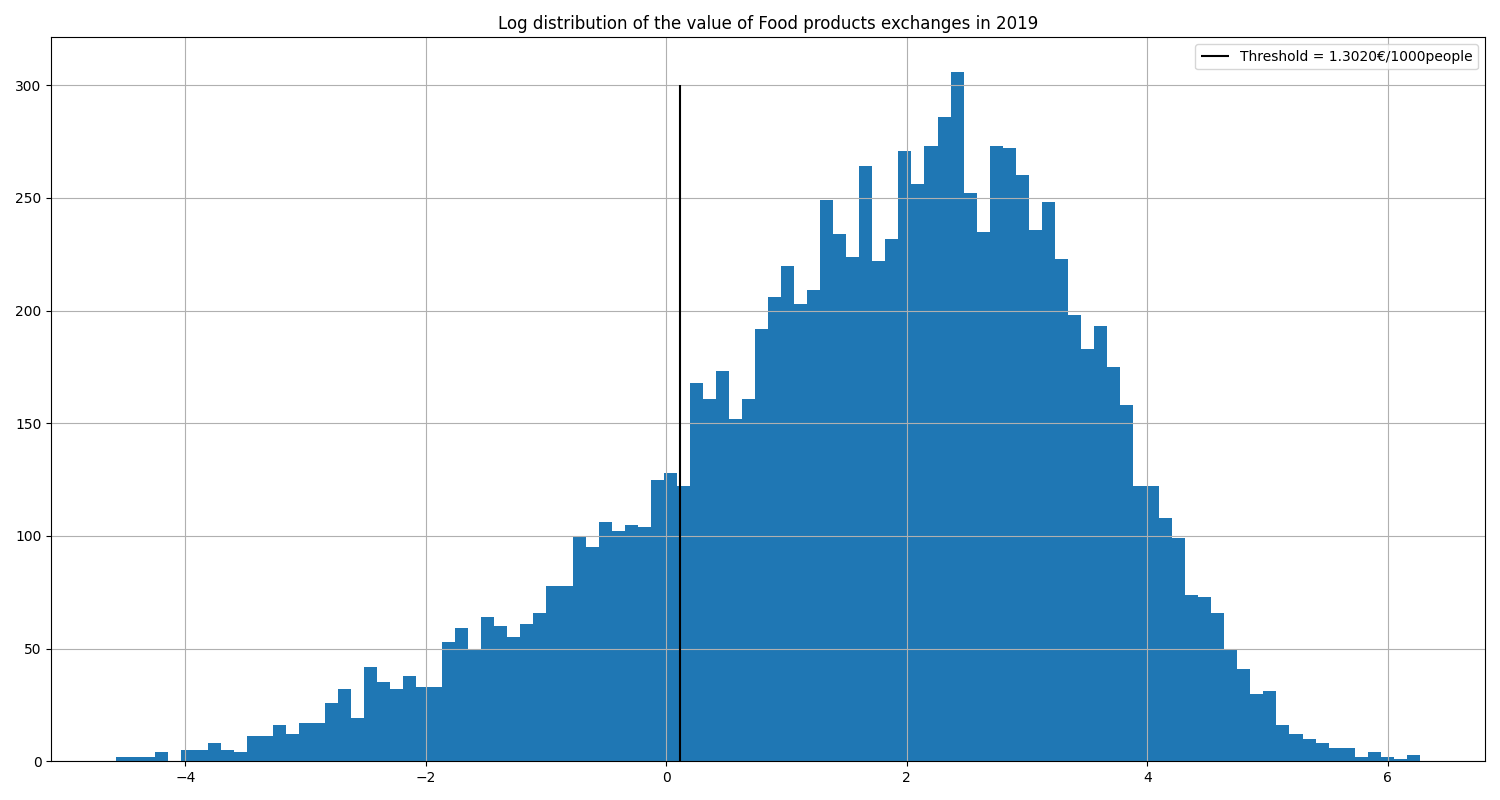
\includegraphics[width=\textwidth]{pics/thresh_complete_y19_p10.png}
    \caption{Distribution of the value of exchanges for the trade network of Food Products in 2019.}
    \label{fig:distrfood19}
\end{figure}

\begin{figure}
    \centering
    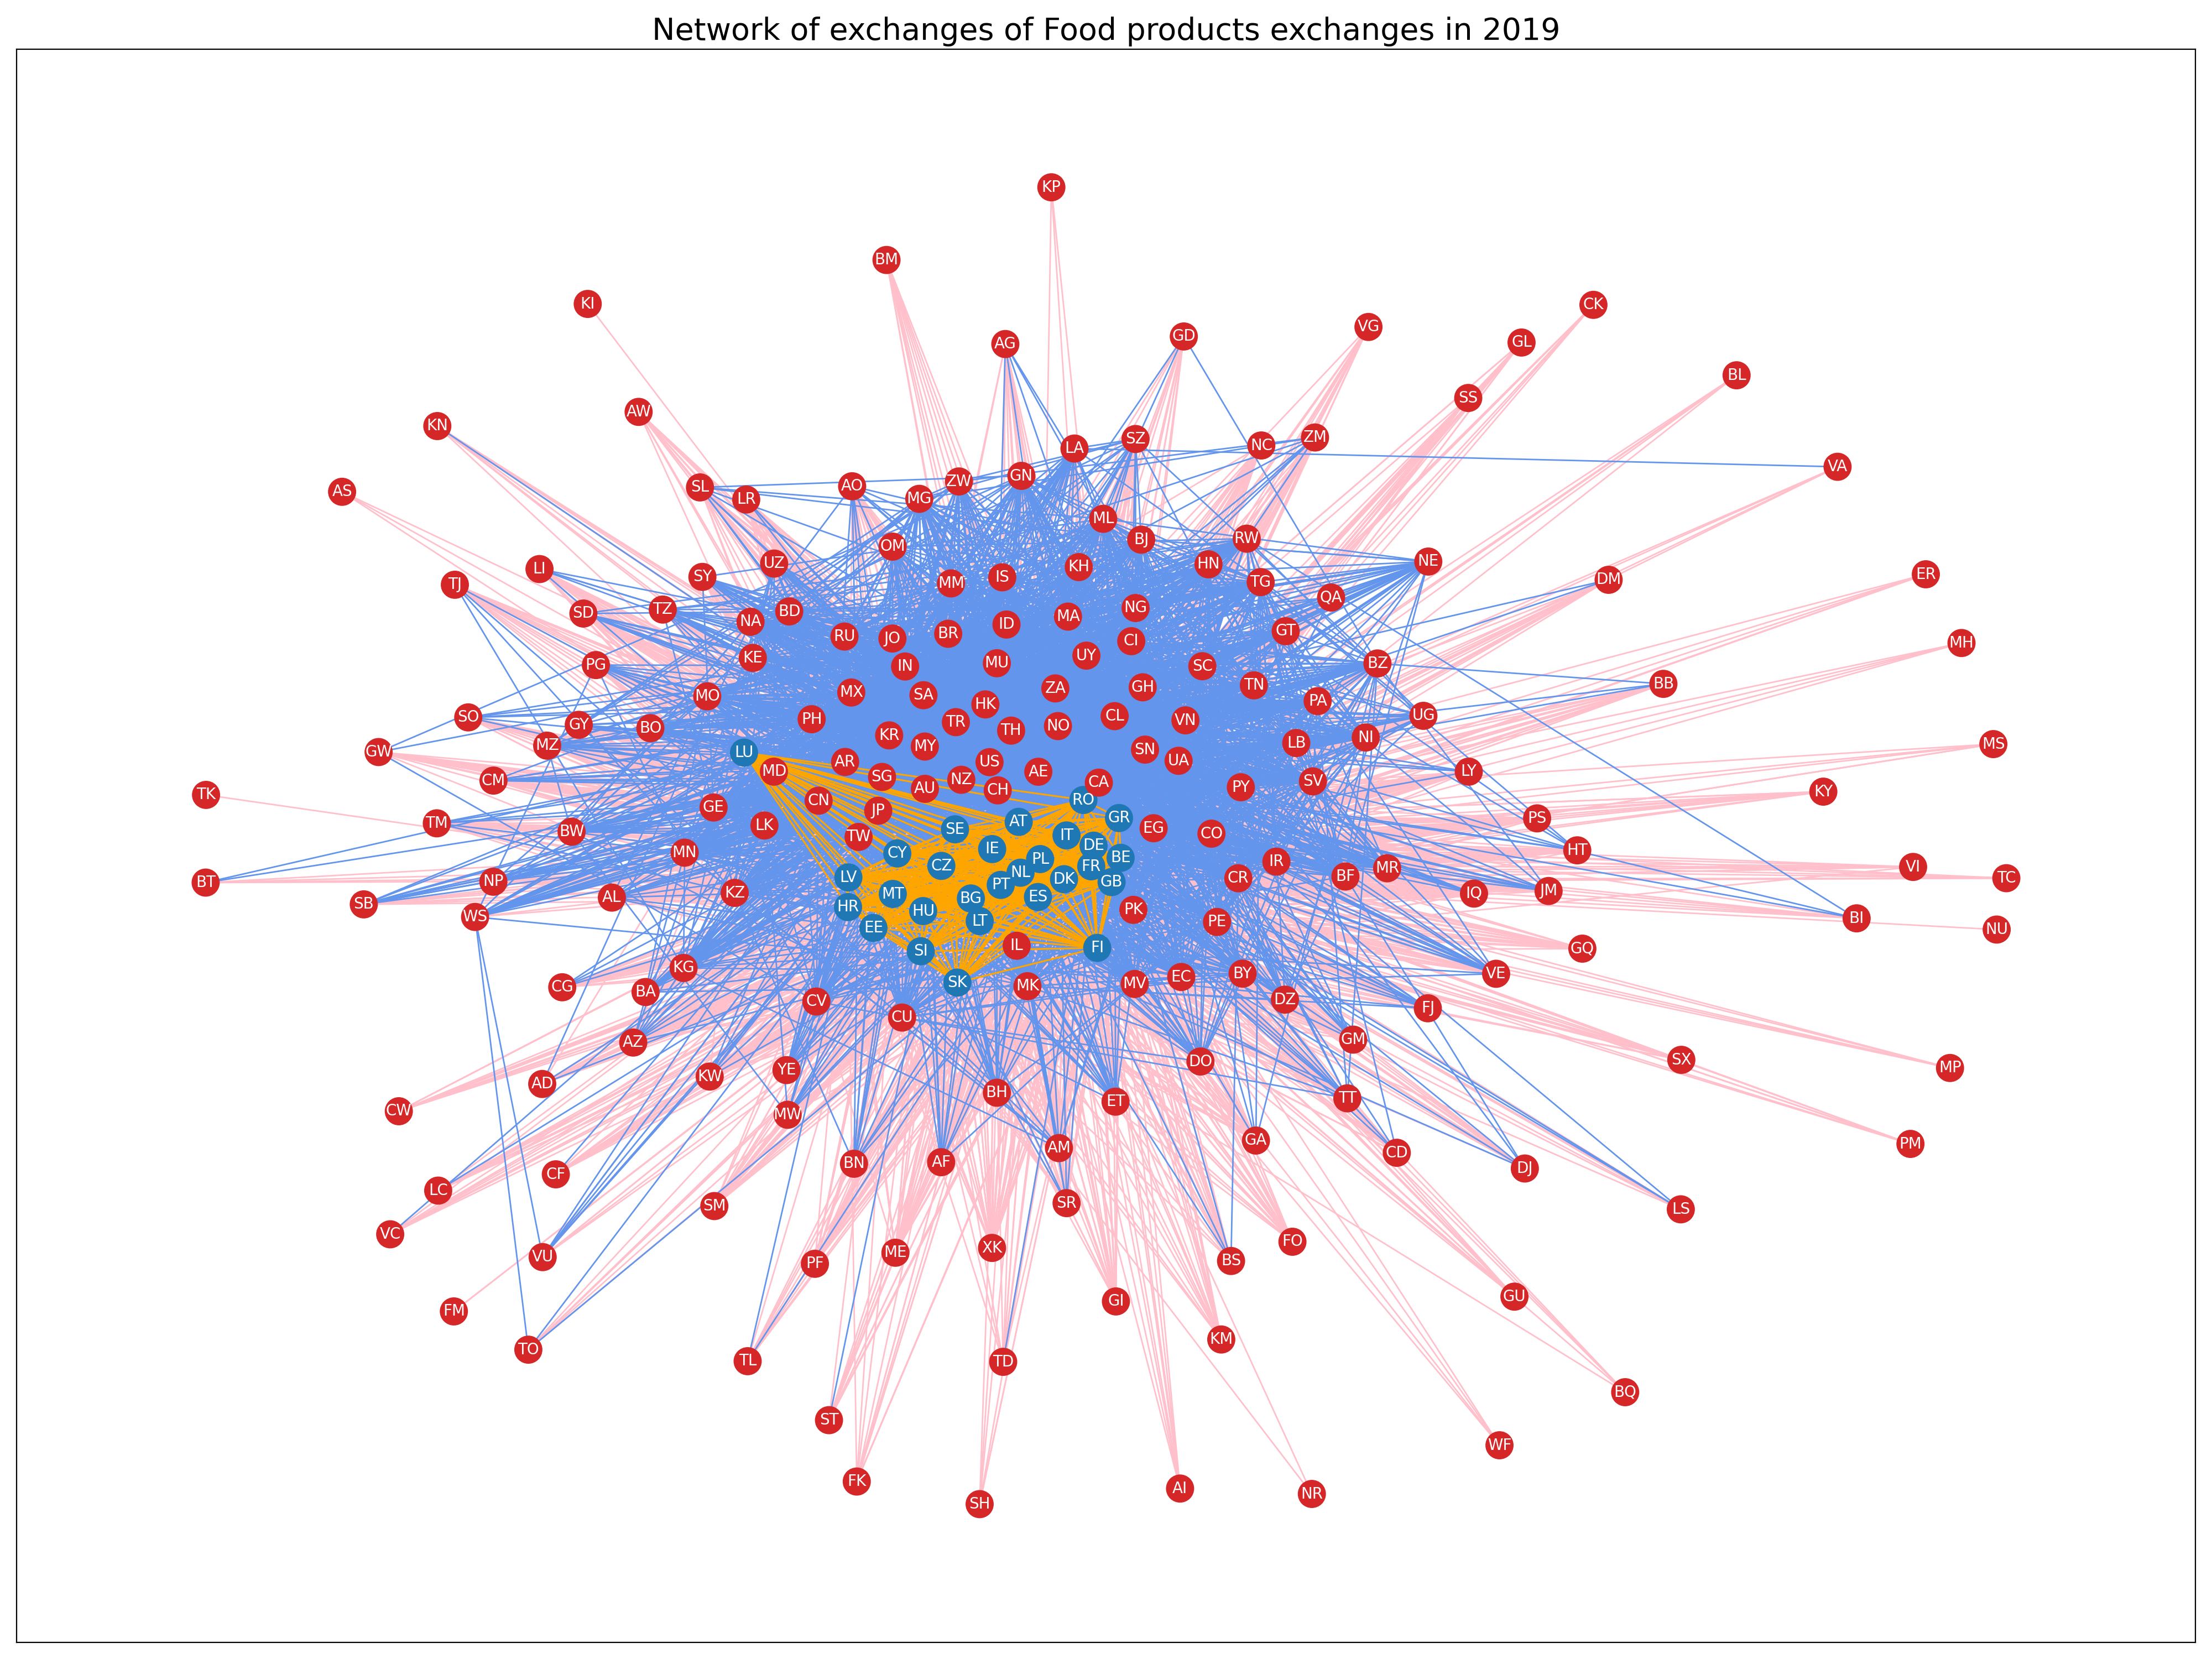
\includegraphics[width=\textwidth]{pics/complete_y19_p10_bin_7.png}
    \caption[Trade network of \textit{Food Products} in 2019, represented as a binary graph.]{Trade network of \textit{Food Products} in 2019, represented as a binary undirected graph using $1.302$ €/1000people as threshold. The color of the node indicates EU countries (\textit{blue}) and non-EU (\textit{red}); the color of the edge is \textit{orange} for intra-EU exchanges, \textit{pink} for EU - non-EU exchanges and \textit{azure} for extra-EU exchanges.}
    \label{fig:foodbingraph}
\end{figure}
% Methods and Analysis chapter
\chapter{Methods and Analysis chapter}
Take my thesis and copy the style, however, basically what you did and how you did it 
So 
\begin{itemize}
    \item Each method \& analysis has its section
    \item Draw some conclusions about this (here \textbf{technical} ones!)
\end{itemize}


% Scenarios and insights
\chapter{Scenarios and Insights chapter}
Miao
\section{Scenarios and Insights section}
Ciao

% \bibliographystyle{alpha}
\printbibliography

\appendix
\chapter{Tables}

\pagebreak
\section{Nomenclatures}

\begin{tabular}{l|c}%
    \bfseries Code & \bfseries Description% specify table head
    % \csvreader[head to column names]{cpa21_l2.csv}{}% use head of csv as column names
    % {\\\hline\Code & \Description}% specify your coloumns here
\end{tabular}

\pagebreak
% \section{ISO Country Codes}
% \resizebox{1.0\textwidth}{!}
{\tiny%\tabcolsep=3pt
\begin{longtable}{lp{5cm}||lp{5cm}}
\caption{Conversion table of country names from ISO 2 codes.\label{tab:iso2}}

\toprule
ISO 2 CODE & COUNTRY NAME & ISO 2 CODE & COUNTRY NAME \\
\midrule
\endfirsthead

\toprule
ISO 2 CODE & COUNTRY NAME & ISO 2 CODE & COUNTRY NAME \\
\midrule
\endhead
\midrule
\multicolumn{4}{r}{{Continued on next page}} \\
\midrule
\endfoot

\bottomrule
\endlastfoot
 AD & Andorra & MG & Madagascar \\
 AE & United Arab Emirates & MH & Marshall Islands \\
 AF & Afghanistan & MK & North Macedonia \\
 AG & Antigua and Barbuda & ML & Mali \\
 AI & Anguilla & MM & Myanmar \\
 AL & Albania & MN & Mongolia \\
 AM & Armenia & MO & Macao \\
 AN & NL Antilles & MP & Northern Mariana Islands \\
 AO & Angola & MQ & Martinique \\
 AQ & Antarctica & MR & Mauritania \\
 AR & Argentina & MS & Montserrat \\
 AS & American Samoa & MT & Malta \\
 AT & Austria & MU & Mauritius \\
 AU & Australia & MV & Maldives \\
 AW & Aruba & MW & Malawi \\
 AZ & Azerbaijan & MX & Mexico \\
 BA & Bosnia-Herzegovina & MY & Malaysia \\
 BB & Barbados & MZ & Mozambique \\
 BD & Bangladesh & NA & Namibia \\
 BE & Belgium and Luxembourg & NC & New Caledonia \\
 BE & Belgium & NE & Niger \\
 BF & Burkina Faso & NF & Norfolk Islands \\
 BG & Bulgaria & NG & Nigeria \\
 BH & Bahrain & NI & Nicaragua \\
 BI & Burundi & NL & Netherlands \\
 BJ & Benin & NO & Norway \\
 BL & St. Barthélemy & NP & Nepal \\
 BM & Bermuda & NR & Nauru \\
 BN & Brunei Darussalam & NU & Niue \\
 BO & Bolivia & NZ & New Zealand \\
 BQ & Bonaire, Sint Eustatius and Saba & OM & Oman \\
 BR & Brazil & PA & Panama \\
 BS & Bahamas & PE & Peru \\
 BT & Bhutan & PF & French Polynesia \\
 BV & Bouvet Island & PG & Papua New Guinea \\
 BW & Botswana & PH & Philippines \\
 BY & Belarus & PK & Pakistan \\
 BZ & Belize & PL & Poland \\
 CA & Canada & PM & St Pierre and Miquelon \\
 CC & Coco Islands & PN & Pitcairn \\
 CD & Congo, Democratic Republic of & PS & Occupied Palestinian Territory \\
 CF & Central African Republic & PT & Portugal \\
 CG & Congo & PW & Palau \\
 CH & Switzerland & PY & Paraguay \\
 CI & Côte d'Ivoire & PZ & Panama Canal \\
 CK & Cook Islands & QA & Qatar \\
 CL & Chile & QP & High Seas \\
 CM & Cameroon & QQ & Stores and Provisions \\
 CN & China & QR & Stores and Provisions Intra \\
 CO & Colombia & QR & Stores and Provisions within the framework of Intra-EU trade \\
 CR & Costa Rica & QS & Stores and Provisions Extra \\
 CS & Czechoslovakia & QS & Stores and Provisions within the framework of trade with third countries \\
 CS & Serbia and Montenegro & QT & West Indies \\
 CU & Cuba & QU & Countries and territories not determined \\
 CV & Cape Verde & QU & Countries and territories not specified \\
 CW & Curacao & QV & Countries and territories not specified within the framework of Intra\_EU trade \\
 CX & Christmas Islands & QW & Countries and territories not specified within the framework of trade with third countries \\
 CY & Cyprus & QX & Countries and territories not specified for commercial or military reasons \\
 CZ & Czechia & QY & Secret countries Intra \\
 DD & Germany, Democratic Republic of & QY & Countries and territories not specified for commercial or military reasons in the framework of Intra\_EU trade \\
 DE & Germany & QZ & Secret countries Extra \\
 DJ & Djibouti & QZ & Countries and territories not specified for commercial or military reasons in the framework of trade with third countries \\
 DK & Denmark & RE & Reunion \\
 DM & Dominica & RO & Romania \\
 DO & Dominican Republic & RU & Russian Federation \\
 DZ & Algeria & RW & Rwanda \\
 EC & Ecuador & SA & Saudi Arabia \\
 EE & Estonia & SB & Solomon Islands \\
 EG & Egypt & SC & Seychelles \\
 EH & Ceuta and Melilla, Spanish Sahara & SD & Sudan \\
 EH & Western Sahara & SE & Sweden \\
 ER & Eritrea & SG & Singapore \\
 ES & Spain & SH & St Helena, Ascension and Tristan Da Cunha \\
 ET & Ethiopia & SI & Slovenia \\
 FI & Finland & SJ & Svalbard \\
 FJ & Fiji & SK & Slovakia \\
 FK & Falkland Islands & SL & Sierra Leone \\
 FK & Falkland Islands (Malvinas) & SM & San Marino \\
 FM & Micronesia, Federated states of & SN & Senegal \\
 FO & Faroe Islands & SO & Somalia \\
 FR & France & SR & Suriname \\
 GA & Gabon & SS & South Sudan \\
 GB & United Kingdom & ST & Sao Tome and Principe \\
 GD & Grenada & SU & Soviet Union \\
 GE & Georgia & SV & El Salvador \\
 GF & French Guiana & SX & Sint Marteen (Dutch part) \\
 GH & Ghana & SY & Syrian Arab Republic \\
 GI & Gibraltar & SZ & Swaziland \\
 GL & Greenland & TC & Turks and Caicos Islands \\
 GM & Gambia & TD & Chad \\
 GN & Guinea & TF & French Southern Territories \\
 GP & Guadeloupe & TG & Togo \\
 GQ & Equatorial Guinea & TH & Thailand \\
 GR & Greece & TJ & Tajikistan \\
 GS & South Georgia and South Sandwich Islands & TK & Tokelau \\
 GT & Guatemala & TL & Timor-Leste \\
 GU & Guam & TM & Turkmenistan \\
 GW & Guinea-Bissau & TN & Tunisia \\
 GY & Guyana & TO & Tonga \\
 HK & Hong Kong & TP & Portugese Timor \\
 HM & Heard Islands and McDonald Islands & TP & East Timor \\
 HN & Honduras & TR & Turkey \\
 HR & Croatia & TT & Trinidad and Tobago \\
 HT & Haiti & TV & Tuvalu \\
 HU & Hungary & TW & Taiwan \\
 ID & Indonesia & TZ & Tanzania, United Republic of \\
 IE & Ireland & UA & Ukraine \\
 IL & Israel & UG & Uganda \\
 IN & India & UM & United States Minor Outlying Islands \\
 IO & British Indian Ocean Territory & US & United States \\
 IQ & Iraq & UY & Uruguay \\
 IR & Iran, Islamic Republic of & UZ & Uzbekistan \\
 IS & Iceland & VA & Holy See (Vatican City State) \\
 IT & Italy & VC & St Vincent and the Grenadines \\
 JM & Jamaica & VD & North Vietnam \\
 JO & Jordan & VE & Venezuela, Bolivarian Republic of \\
 JP & Japan & VG & Virgin Islands, British \\
 KE & Kenya & VI & Virgin Islands, United States \\
 KG & Kyrgyzstan & VN & Viet Nam \\
 KG & Kyrgyz, Republic & VU & Vanuatu \\
 KH & Cambodia & WF & Wallis and Futuna \\
 KI & Kiribati & WS & Samoa \\
 KM & Comoros & XA & American Oceania \\
 KN & St Kitts and Nevis & XB & Canary Islands \\
 KP & Korea, Democratic People's Republic of & XC & Ceuta \\
 KR & Korea, Republic of & XI & United Kingdom (Northern Ireland) \\
 KW & Kuwait & XK & Kosovo \\
 KY & Cayman Islands & XL & Melilla \\
 KZ & Kazakhstan & XM & Montenegro \\
 LA & Lao People's Democratic Republic & XO & Australian Oceania \\
 LB & Lebanon & XP & West Bank and Gaza Strip \\
 LC & St Lucia & XR & Polar Regions \\
 LI & Liechtenstein & XS & Serbia \\
 LK & Sri Lanka & XU & United Kingdom (excluding Northern Ireland) \\
 LR & Liberia & XZ & New Zealand Oceania \\
 LS & Lesotho & YD & South Yemen \\
 LT & Lithuania & YE & Yemen \\
 LU & Luxembourg & YT & Mayotte \\
 LV & Latvia & YU & Yugoslavia \\
 LY & Libya & ZA & South Africa \\
 MA & Morocco & ZM & Zambia \\
 MD & Moldova & ZW & Zimbabwe \\
 MD & Moldova, Republic of & ZZ & No data, work code \\
 ME & Montenegro &  &  \\
\end{longtable}
}

\pagebreak
\section{UN Population}\label{app:unpop}
{\tiny
\begin{longtable}{rlllrrrrr}
\caption{Population according to UN estimates updated at 2022.\label{tab:unpop}}
\toprule
 ID & iso2 & iso3 & Country & 2000 & 2005 & 2010 & 2015 & 2020 \\
\midrule
\endfirsthead

\toprule
 ID & iso2 & iso3 & Country & 2000 & 2005 & 2010 & 2015 & 2020 \\
\midrule
\endhead
\midrule
\multicolumn{9}{r}{{Continued on next page}} \\
\midrule
\endfoot

\bottomrule
\endlastfoot
 4 & AF & AFG & Afghanistan & 19542.982 & 24411.191 & 28189.672 & 33753.499 & 38972.230 \\
 8 & AL & ALB & Albania & 3182.021 & 3032.634 & 2913.399 & 2882.481 & 2866.849 \\
 12 & DZ & DZA & Algeria & 30774.621 & 32956.690 & 35856.344 & 39543.154 & 43451.666 \\
 16 & AS & ASM & American Samoa & 58.230 & 57.254 & 54.849 & 51.368 & 46.189 \\
 20 & AD & AND & Andorra & 66.097 & 79.826 & 71.519 & 71.746 & 77.700 \\
 24 & AO & AGO & Angola & 16394.062 & 19450.959 & 23364.185 & 28127.721 & 33428.486 \\
 28 & AG & ATG & Antigua and Barbuda & 75.055 & 79.869 & 85.695 & 89.941 & 92.664 \\
 31 & AZ & AZE & Azerbaijan & 8190.337 & 8656.237 & 9237.202 & 9863.480 & 10284.951 \\
 32 & AR & ARG & Argentina & 37070.774 & 39070.501 & 41100.123 & 43257.065 & 45036.032 \\
 36 & AU & AUS & Australia & 19017.963 & 20171.731 & 22019.168 & 23820.236 & 25670.051 \\
 40 & AT & AUT & Austria & 8010.428 & 8227.034 & 8362.829 & 8642.421 & 8907.777 \\
 44 & BS & BHS & Bahamas & 325.014 & 347.804 & 373.272 & 392.697 & 406.471 \\
 48 & BH & BHR & Bahrain & 711.442 & 901.921 & 1213.645 & 1362.142 & 1477.469 \\
 50 & BD & BGD & Bangladesh & 129193.327 & 140912.590 & 148391.139 & 157830.000 & 167420.951 \\
 51 & AM & ARM & Armenia & 3168.523 & 3047.246 & 2946.293 & 2878.595 & 2805.608 \\
 52 & BB & BRB & Barbados & 264.657 & 269.477 & 274.711 & 278.083 & 280.693 \\
 56 & BE & BEL & Belgium & 10264.343 & 10516.978 & 10877.947 & 11248.303 & 11561.717 \\
 60 & BM & BMU & Bermuda & 61.371 & 62.959 & 63.447 & 63.144 & 64.031 \\
 64 & BT & BTN & Bhutan & 587.207 & 663.323 & 705.516 & 743.274 & 772.506 \\
 68 & BO & BOL & Bolivia (Plurinational State of) & 8592.656 & 9377.388 & 10223.270 & 11090.085 & 11936.162 \\
 70 & BA & BIH & Bosnia and Herzegovina & 4179.350 & 4094.297 & 3811.088 & 3524.324 & 3318.407 \\
 72 & BW & BWA & Botswana & 1726.985 & 1892.807 & 2091.664 & 2305.171 & 2546.402 \\
 76 & BR & BRA & Brazil & 175873.720 & 186797.334 & 196353.492 & 205188.205 & 213196.304 \\
 84 & BZ & BLZ & Belize & 240.406 & 280.375 & 322.106 & 359.871 & 394.921 \\
 90 & SB & SLB & Solomon Islands & 429.978 & 482.486 & 540.394 & 612.660 & 691.191 \\
 92 & VG & VGB & British Virgin Islands & 20.104 & 23.497 & 27.556 & 29.366 & 30.910 \\
 96 & BN & BRN & Brunei Darussalam & 333.926 & 366.717 & 396.053 & 421.437 & 441.725 \\
 100 & BG & BGR & Bulgaria & 8097.691 & 7815.221 & 7592.273 & 7309.253 & 6979.175 \\
 104 & MM & MMR & Myanmar & 45538.332 & 47724.471 & 49390.988 & 51483.949 & 53423.198 \\
 108 & BI & BDI & Burundi & 6307.659 & 7388.874 & 9126.605 & 10727.148 & 12220.227 \\
 112 & BY & BLR & Belarus & 10256.483 & 9935.163 & 9731.427 & 9700.609 & 9633.740 \\
 116 & KH & KHM & Cambodia & 12118.841 & 13246.583 & 14363.532 & 15417.523 & 16396.860 \\
 120 & CM & CMR & Cameroon & 15091.594 & 17275.171 & 19878.036 & 23012.646 & 26491.087 \\
 124 & CA & CAN & Canada & 30683.313 & 32215.916 & 33963.412 & 35732.126 & 37888.705 \\
 132 & CV & CPV & Cabo Verde & 458.251 & 492.827 & 521.212 & 552.166 & 582.640 \\
 136 & KY & CYM & Cayman Islands & 39.658 & 46.727 & 54.074 & 60.911 & 67.311 \\
 140 & CF & CAF & Central African Republic & 3759.170 & 4208.834 & 4660.067 & 4819.333 & 5343.020 \\
 144 & LK & LKA & Sri Lanka & 18776.371 & 19673.866 & 20668.557 & 21336.697 & 21715.079 \\
 148 & TD & TCD & Chad & 8259.137 & 10005.012 & 11894.727 & 14140.274 & 16644.701 \\
 152 & CL & CHL & Chile & 15351.799 & 16175.311 & 17004.162 & 17870.124 & 19300.315 \\
 156 & CN & CHN & China & 1264099.069 & 1304887.562 & 1348191.368 & 1393715.448 & 1424929.781 \\
 158 & TW & TWN & China, Taiwan Province of China & 22194.731 & 22796.306 & 23083.083 & 23512.136 & 23821.464 \\
 170 & CO & COL & Colombia & 39215.135 & 42220.940 & 44816.108 & 47119.728 & 50930.662 \\
 174 & KM & COM & Comoros & 536.758 & 592.683 & 656.024 & 730.216 & 806.166 \\
 175 & YT & MYT & Mayotte & 159.215 & 187.142 & 211.786 & 249.545 & 305.587 \\
 178 & CG & COG & Congo & 3134.030 & 3672.839 & 4437.884 & 5064.386 & 5702.174 \\
 180 & CD & COD & Democratic Republic of the Congo & 48616.317 & 56550.247 & 66391.257 & 78656.904 & 92853.164 \\
 184 & CK & COK & Cook Islands & 15.897 & 15.146 & 17.212 & 17.695 & 17.029 \\
 188 & CR & CRI & Costa Rica & 3979.193 & 4315.887 & 4622.252 & 4895.242 & 5123.105 \\
 191 & HR & HRV & Croatia & 4548.434 & 4429.681 & 4368.682 & 4254.815 & 4096.869 \\
 192 & CU & CUB & Cuba & 11105.791 & 11246.114 & 11290.417 & 11339.894 & 11300.698 \\
 196 & CY & CYP & Cyprus & 948.237 & 1037.062 & 1129.686 & 1187.280 & 1237.537 \\
 203 & CZ & CZE & Czechia & 10234.710 & 10280.113 & 10464.749 & 10523.798 & 10530.953 \\
 204 & BJ & BEN & Benin & 6998.023 & 8149.419 & 9445.710 & 10932.783 & 12643.123 \\
 208 & DK & DNK & Denmark & 5340.655 & 5436.313 & 5550.849 & 5677.796 & 5825.641 \\
 212 & DM & DMA & Dominica & 68.346 & 68.674 & 68.755 & 70.007 & 71.995 \\
 214 & DO & DOM & Dominican Republic & 8540.791 & 9164.768 & 9775.755 & 10405.832 & 10999.664 \\
 218 & EC & ECU & Ecuador & 12626.507 & 13770.012 & 14989.585 & 16195.902 & 17588.595 \\
 222 & SV & SLV & El Salvador & 5958.482 & 6037.817 & 6114.034 & 6231.066 & 6292.731 \\
 226 & GQ & GNQ & Equatorial Guinea & 684.977 & 864.726 & 1094.524 & 1346.973 & 1596.049 \\
 231 & ET & ETH & Ethiopia & 67031.867 & 77469.940 & 89237.791 & 102471.895 & 117190.911 \\
 232 & ER & ERI & Eritrea & 2392.880 & 2831.732 & 3147.727 & 3340.006 & 3555.868 \\
 233 & EE & EST & Estonia & 1396.877 & 1354.662 & 1331.535 & 1314.657 & 1329.444 \\
 234 & FO & FRO & Faroe Islands & 45.660 & 48.291 & 48.410 & 48.816 & 52.415 \\
 238 & FK & FLK & Falkland Islands (Malvinas) & 3.080 & 3.204 & 3.187 & 3.408 & 3.747 \\
 242 & FJ & FJI & Fiji & 832.509 & 874.923 & 905.169 & 917.200 & 920.422 \\
 246 & FI & FIN & Finland & 5176.209 & 5246.071 & 5363.271 & 5479.461 & 5529.468 \\
 250 & FR & FRA & France & 58665.453 & 60510.079 & 62444.567 & 63809.769 & 64480.053 \\
 254 & GF & GUF & French Guiana & 164.351 & 201.259 & 228.453 & 257.026 & 290.969 \\
 258 & PF & PYF & French Polynesia & 250.927 & 271.060 & 283.788 & 291.787 & 301.920 \\
 262 & DJ & DJI & Djibouti & 742.033 & 830.861 & 919.199 & 1006.259 & 1090.156 \\
 266 & GA & GAB & Gabon & 1272.935 & 1458.353 & 1711.105 & 2028.517 & 2292.573 \\
 268 & GE & GEO & Georgia & 4265.172 & 3961.182 & 3836.831 & 3771.132 & 3765.912 \\
 270 & GM & GMB & Gambia & 1437.539 & 1660.368 & 1937.275 & 2253.133 & 2573.995 \\
 275 & PS & PSE & State of Palestine & 3139.954 & 3541.193 & 3992.278 & 4484.614 & 5019.401 \\
 276 & DE & DEU & Germany & 81551.677 & 81212.168 & 81325.090 & 82073.226 & 83328.988 \\
 288 & GH & GHA & Ghana & 19665.502 & 22496.951 & 25574.719 & 28870.939 & 32180.401 \\
 292 & GI & GIB & Gibraltar & 27.741 & 29.155 & 31.262 & 32.520 & 32.709 \\
 296 & KI & KIR & Kiribati & 88.826 & 98.164 & 107.995 & 116.707 & 126.463 \\
 300 & GR & GRC & Greece & 11038.109 & 11113.448 & 11033.783 & 10806.641 & 10512.232 \\
 304 & GL & GRL & Greenland & 56.184 & 56.887 & 56.351 & 55.895 & 56.026 \\
 308 & GD & GRD & Grenada & 107.432 & 110.254 & 114.039 & 118.980 & 123.663 \\
 312 & GP & GLP & Guadeloupe & 424.067 & 403.233 & 403.072 & 399.089 & 395.642 \\
 316 & GU & GUM & Guam & 160.188 & 164.430 & 164.905 & 167.978 & 169.231 \\
 320 & GT & GTM & Guatemala & 11735.894 & 13132.814 & 14543.121 & 16001.107 & 17362.718 \\
 324 & GN & GIN & Guinea & 8336.967 & 9140.114 & 10270.728 & 11625.998 & 13205.153 \\
 328 & GY & GUY & Guyana & 759.051 & 759.709 & 747.932 & 755.031 & 797.202 \\
 332 & HT & HTI & Haiti & 8360.225 & 9111.900 & 9842.880 & 10563.757 & 11306.801 \\
 336 & VA & VAT & Holy See & 0.651 & 0.628 & 0.596 & 0.564 & 0.520 \\
 340 & HN & HND & Honduras & 6656.725 & 7564.613 & 8450.933 & 9294.505 & 10121.763 \\
 344 & HK & HKG & China, Hong Kong SAR & 6731.195 & 6936.874 & 7132.438 & 7399.838 & 7500.958 \\
 348 & HU & HUN & Hungary & 10202.055 & 10073.525 & 9986.825 & 9844.246 & 9750.573 \\
 352 & IS & ISL & Iceland & 281.462 & 297.029 & 318.333 & 331.060 & 366.669 \\
 356 & IN & IND & India & 1059633.675 & 1154638.713 & 1240613.620 & 1322866.505 & 1396387.127 \\
 360 & ID & IDN & Indonesia & 214072.421 & 228805.144 & 244016.173 & 259091.970 & 271857.970 \\
 364 & IR & IRN & Iran (Islamic Republic of) & 65544.383 & 70182.594 & 75373.855 & 81790.841 & 87290.193 \\
 368 & IQ & IRQ & Iraq & 24628.858 & 28698.684 & 31264.875 & 37757.813 & 42556.984 \\
 372 & IE & IRL & Ireland & 3768.950 & 4121.216 & 4524.585 & 4665.760 & 4946.119 \\
 376 & IL & ISR & Israel & 6116.958 & 6714.124 & 7328.445 & 8007.778 & 8757.489 \\
 380 & IT & ITA & Italy & 56966.397 & 58199.876 & 59822.450 & 60232.906 & 59500.579 \\
 384 & CI & CIV & Côte d'Ivoire & 16799.670 & 18970.215 & 21120.042 & 23596.741 & 26811.790 \\
 388 & JM & JAM & Jamaica & 2612.205 & 2676.863 & 2733.896 & 2794.445 & 2820.436 \\
 392 & JP & JPN & Japan & 126803.861 & 127798.373 & 128105.431 & 127250.933 & 125244.761 \\
 398 & KZ & KAZ & Kazakhstan & 15236.253 & 15656.248 & 16627.837 & 17835.909 & 18979.243 \\
 400 & JO & JOR & Jordan & 5056.174 & 5678.534 & 6931.258 & 9494.246 & 10928.721 \\
 404 & KE & KEN & Kenya & 30851.606 & 35843.010 & 41517.895 & 46851.488 & 51985.780 \\
 408 & KP & PRK & Dem. People's Republic of Korea & 23367.059 & 24100.982 & 24686.435 & 25258.015 & 25867.467 \\
 410 & KR & KOR & Republic of Korea & 46788.591 & 47889.573 & 48813.042 & 50994.401 & 51844.690 \\
 412 & XK & XKX & Kosovo (under UNSC res. 1244) & 1823.286 & 1825.050 & 1792.563 & 1759.122 & 1670.698 \\
 414 & KW & KWT & Kuwait & 1934.901 & 2235.403 & 2943.356 & 3908.743 & 4360.444 \\
 417 & KG & KGZ & Kyrgyzstan & 4935.182 & 5193.114 & 5483.774 & 5914.980 & 6424.874 \\
 418 & LA & LAO & Lao People's Democratic Republic & 5430.853 & 5852.970 & 6323.418 & 6787.419 & 7319.399 \\
 422 & LB & LBN & Lebanon & 4320.642 & 4643.044 & 4995.800 & 6398.940 & 5662.923 \\
 426 & LS & LSO & Lesotho & 1998.630 & 1977.424 & 2022.747 & 2118.521 & 2254.100 \\
 428 & LV & LVA & Latvia & 2392.530 & 2233.157 & 2101.530 & 1991.955 & 1897.052 \\
 430 & LR & LBR & Liberia & 2895.224 & 3266.318 & 4019.956 & 4612.329 & 5087.584 \\
 434 & LY & LBY & Libya & 5154.790 & 5837.986 & 6491.988 & 6192.235 & 6653.942 \\
 438 & LI & LIE & Liechtenstein & 33.026 & 34.603 & 35.926 & 37.355 & 38.756 \\
 440 & LT & LTU & Lithuania & 3599.637 & 3373.533 & 3139.019 & 2963.765 & 2820.267 \\
 442 & LU & LUX & Luxembourg & 435.628 & 464.860 & 507.070 & 569.408 & 630.399 \\
 446 & MO & MAC & China, Macao SAR & 431.896 & 488.619 & 557.297 & 615.239 & 676.283 \\
 450 & MG & MDG & Madagascar & 16216.431 & 18792.171 & 21731.053 & 24850.912 & 28225.177 \\
 454 & MW & MWI & Malawi & 11229.387 & 12755.648 & 14718.422 & 16938.942 & 19377.061 \\
 458 & MY & MYS & Malaysia & 22945.150 & 25923.536 & 28717.731 & 31068.833 & 33199.993 \\
 462 & MV & MDV & Maldives & 282.507 & 307.018 & 361.575 & 435.582 & 514.438 \\
 466 & ML & MLI & Mali & 11239.101 & 13180.551 & 15529.181 & 18112.907 & 21224.040 \\
 470 & MT & MLT & Malta & 399.212 & 410.208 & 418.755 & 456.579 & 515.358 \\
 474 & MQ & MTQ & Martinique & 432.543 & 400.370 & 392.181 & 383.515 & 370.391 \\
 478 & MR & MRT & Mauritania & 2695.003 & 3012.360 & 3419.461 & 3946.220 & 4498.604 \\
 480 & MU & MUS & Mauritius & 1215.930 & 1258.048 & 1283.330 & 1293.153 & 1297.828 \\
 484 & MX & MEX & Mexico & 97873.442 & 105442.402 & 112532.401 & 120149.897 & 125998.302 \\
 492 & MC & MCO & Monaco & 32.465 & 32.141 & 33.178 & 36.760 & 36.922 \\
 496 & MN & MNG & Mongolia & 2450.979 & 2559.255 & 2702.520 & 2964.749 & 3294.335 \\
 498 & MD & MDA & Republic of Moldova & 4251.573 & 4001.382 & 3678.186 & 3277.388 & 3084.847 \\
 499 & ME & MNE & Montenegro & 633.324 & 632.875 & 631.044 & 633.966 & 629.048 \\
 500 & MS & MSR & Montserrat & 5.138 & 4.693 & 4.938 & 5.059 & 4.500 \\
 504 & MA & MAR & Morocco & 28554.415 & 30431.902 & 32464.865 & 34680.458 & 36688.772 \\
 508 & MZ & MOZ & Mozambique & 17768.505 & 20211.114 & 23073.723 & 26843.246 & 31178.239 \\
 512 & OM & OMN & Oman & 2344.253 & 2515.192 & 2881.914 & 4191.776 & 4543.399 \\
 516 & NA & NAM & Namibia & 1819.141 & 1962.865 & 2099.271 & 2282.704 & 2489.098 \\
 520 & NR & NRU & Nauru & 10.377 & 10.318 & 10.241 & 11.185 & 12.315 \\
 524 & NP & NPL & Nepal & 24559.500 & 26285.110 & 27161.567 & 27610.325 & 29348.627 \\
 528 & NL & NLD & Netherlands & 15899.135 & 16261.831 & 16617.117 & 17041.107 & 17434.557 \\
 531 & CW & CUW & Curaçao & 141.424 & 147.263 & 159.380 & 169.572 & 189.288 \\
 533 & AW & ABW & Aruba & 89.101 & 94.483 & 100.341 & 104.257 & 106.585 \\
 534 & SX & SXM & Sint Maarten (Dutch part) & 30.489 & 31.494 & 33.034 & 40.205 & 43.621 \\
 535 & BQ & BES & Bonaire, Sint Eustatius and Saba & 13.960 & 16.724 & 20.224 & 23.164 & 26.153 \\
 540 & NC & NCL & New Caledonia & 221.537 & 242.141 & 261.426 & 283.032 & 286.403 \\
 548 & VU & VUT & Vanuatu & 192.074 & 217.632 & 245.453 & 276.438 & 311.685 \\
 554 & NZ & NZL & New Zealand & 3855.266 & 4132.781 & 4346.338 & 4590.590 & 5061.133 \\
 558 & NI & NIC & Nicaragua & 5123.222 & 5454.678 & 5855.734 & 6298.598 & 6755.895 \\
 562 & NE & NER & Niger & 11622.665 & 13855.221 & 16647.543 & 20128.124 & 24333.639 \\
 566 & NG & NGA & Nigeria & 122851.984 & 140490.722 & 160952.853 & 183995.785 & 208327.405 \\
 570 & NU & NIU & Niue & 2.074 & 1.856 & 1.812 & 1.847 & 1.942 \\
 578 & NO & NOR & Norway & 4491.202 & 4623.689 & 4889.741 & 5190.356 & 5379.839 \\
 580 & MP & MNP & Northern Mariana Islands & 80.338 & 69.025 & 54.087 & 51.514 & 49.587 \\
 583 & FM & FSM & Micronesia (Fed. States of) & 111.709 & 110.940 & 107.588 & 109.462 & 112.106 \\
 584 & MH & MHL & Marshall Islands & 54.224 & 54.337 & 53.416 & 49.410 & 43.413 \\
 585 & PW & PLW & Palau & 19.726 & 19.831 & 18.540 & 17.794 & 17.972 \\
 586 & PK & PAK & Pakistan & 154369.924 & 174372.098 & 194454.498 & 210969.298 & 227196.741 \\
 591 & PA & PAN & Panama & 3001.731 & 3305.868 & 3623.617 & 3957.099 & 4294.396 \\
 598 & PG & PNG & Papua New Guinea & 5508.297 & 6498.818 & 7583.269 & 8682.174 & 9749.640 \\
 600 & PY & PRY & Paraguay & 5123.819 & 5476.878 & 5768.613 & 6177.950 & 6618.695 \\
 604 & PE & PER & Peru & 26654.439 & 28147.267 & 29229.572 & 30711.863 & 33304.756 \\
 608 & PH & PHL & Philippines & 77958.223 & 86261.250 & 94636.700 & 103031.365 & 112190.977 \\
 616 & PL & POL & Poland & 38504.431 & 38575.911 & 38597.353 & 38553.146 & 38428.366 \\
 620 & PT & PRT & Portugal & 10300.626 & 10523.315 & 10588.401 & 10365.435 & 10298.192 \\
 624 & GW & GNB & Guinea-Bissau & 1230.849 & 1379.713 & 1567.220 & 1788.919 & 2015.828 \\
 626 & TL & TLS & Timor-Leste & 878.360 & 969.313 & 1088.486 & 1205.813 & 1299.995 \\
 630 & PR & PRI & Puerto Rico & 3827.108 & 3805.559 & 3717.922 & 3497.335 & 3271.564 \\
 634 & QA & QAT & Qatar & 645.937 & 848.710 & 1713.504 & 2414.573 & 2760.385 \\
 638 & RE & REU & Réunion & 785.424 & 833.656 & 890.130 & 922.495 & 957.822 \\
 642 & RO & ROU & Romania & 21919.876 & 21092.264 & 20335.211 & 19906.079 & 19442.038 \\
 643 & RU & RUS & Russian Federation & 146844.839 & 143800.049 & 143242.599 & 144668.389 & 145617.329 \\
 646 & RW & RWA & Rwanda & 8109.989 & 9026.299 & 10309.031 & 11642.959 & 13146.362 \\
 652 & BL & BLM & Saint Barthélemy & 7.082 & 8.044 & 8.988 & 9.643 & 10.681 \\
 654 & SH & SHN & Saint Helena & 6.024 & 5.532 & 5.321 & 5.497 & 5.420 \\
 659 & KN & KNA & Saint Kitts and Nevis & 45.461 & 46.725 & 47.403 & 47.790 & 47.642 \\
 660 & AI & AIA & Anguilla & 11.047 & 12.128 & 13.172 & 14.525 & 15.585 \\
 662 & LC & LCA & Saint Lucia & 159.500 & 165.386 & 170.935 & 175.623 & 179.237 \\
 663 & MF & MAF & Saint Martin (French part) & 29.610 & 33.452 & 36.458 & 35.020 & 32.553 \\
 666 & PM & SPM & Saint Pierre and Miquelon & 6.274 & 6.115 & 6.052 & 5.978 & 5.906 \\
 670 & VC & VCT & Saint Vincent and the Grenadines & 113.813 & 112.043 & 109.308 & 106.482 & 104.632 \\
 674 & SM & SMR & San Marino & 26.823 & 29.508 & 31.608 & 33.570 & 34.007 \\
 678 & ST & STP & Sao Tome and Principe & 143.714 & 161.680 & 182.138 & 201.124 & 218.641 \\
 682 & SA & SAU & Saudi Arabia & 21547.390 & 24397.644 & 29411.929 & 32749.848 & 35997.107 \\
 686 & SN & SEN & Senegal & 9704.287 & 10974.057 & 12530.121 & 14356.181 & 16436.120 \\
 688 & RS & SRB & Serbia & 7935.022 & 7830.944 & 7653.748 & 7519.496 & 7358.005 \\
 690 & SC & SYC & Seychelles & 80.060 & 85.883 & 92.409 & 99.240 & 105.530 \\
 694 & SL & SLE & Sierra Leone & 4584.067 & 5683.334 & 6436.698 & 7314.773 & 8233.970 \\
 702 & SG & SGP & Singapore & 4053.602 & 4344.637 & 5163.590 & 5650.018 & 5909.869 \\
 703 & SK & SVK & Slovakia & 5376.690 & 5376.242 & 5396.424 & 5424.444 & 5456.681 \\
 704 & VN & VNM & Viet Nam & 79001.142 & 83142.095 & 87411.012 & 92191.398 & 96648.685 \\
 705 & SI & SVN & Slovenia & 1984.339 & 2004.778 & 2057.287 & 2080.862 & 2117.641 \\
 706 & SO & SOM & Somalia & 8721.465 & 10467.292 & 12026.649 & 13763.906 & 16537.016 \\
 710 & ZA & ZAF & South Africa & 46813.266 & 49017.147 & 51784.921 & 55876.504 & 58801.927 \\
 716 & ZW & ZWE & Zimbabwe & 11834.676 & 12224.753 & 12839.771 & 14154.937 & 15669.666 \\
 724 & ES & ESP & Spain & 40741.651 & 43685.374 & 46572.772 & 46431.342 & 47363.807 \\
 728 & SS & SSD & South Sudan & 6114.440 & 7662.654 & 9714.419 & 11194.299 & 10606.227 \\
 729 & SD & SDN & Sudan & 26298.773 & 29540.577 & 33739.933 & 38171.178 & 44440.486 \\
 732 & EH & ESH & Western Sahara & 270.375 & 339.187 & 413.296 & 491.824 & 556.048 \\
 740 & SR & SUR & Suriname & 478.998 & 516.220 & 546.080 & 575.475 & 607.065 \\
 748 & SZ & SWZ & Eswatini & 1030.496 & 1071.886 & 1099.920 & 1133.936 & 1180.655 \\
 752 & SE & SWE & Sweden & 8871.043 & 9051.738 & 9381.729 & 9849.349 & 10368.969 \\
 756 & CH & CHE & Switzerland & 7182.059 & 7428.435 & 7822.435 & 8281.732 & 8638.613 \\
 760 & SY & SYR & Syrian Arab Republic & 16307.654 & 18583.557 & 22337.563 & 19205.178 & 20772.595 \\
 762 & TJ & TJK & Tajikistan & 6272.998 & 6929.145 & 7621.779 & 8524.063 & 9543.207 \\
 764 & TH & THA & Thailand & 63066.603 & 65821.360 & 68270.489 & 70294.397 & 71475.664 \\
 768 & TG & TGO & Togo & 5008.035 & 5711.597 & 6571.855 & 7473.229 & 8442.580 \\
 772 & TK & TKL & Tokelau & 1.666 & 1.429 & 1.367 & 1.454 & 1.827 \\
 776 & TO & TON & Tonga & 102.603 & 105.633 & 107.383 & 106.122 & 105.254 \\
 780 & TT & TTO & Trinidad and Tobago & 1332.203 & 1369.075 & 1410.296 & 1460.177 & 1518.147 \\
 784 & AE & ARE & United Arab Emirates & 3275.333 & 4280.993 & 8481.771 & 8916.899 & 9287.289 \\
 788 & TN & TUN & Tunisia & 9893.316 & 10388.344 & 10895.063 & 11557.779 & 12161.723 \\
 792 & TR & TUR & Türkiye & 64113.547 & 68704.715 & 73195.345 & 79646.178 & 84135.428 \\
 795 & TM & TKM & Turkmenistan & 4569.132 & 4885.775 & 5267.970 & 5766.431 & 6250.438 \\
 796 & TC & TCA & Turks and Caicos Islands & 18.744 & 23.995 & 29.726 & 36.538 & 44.276 \\
 798 & TV & TUV & Tuvalu & 9.638 & 9.912 & 10.550 & 10.877 & 11.069 \\
 800 & UG & UGA & Uganda & 24020.697 & 27946.588 & 32341.728 & 37477.356 & 44404.611 \\
 804 & UA & UKR & Ukraine & 48879.755 & 46912.610 & 45683.020 & 44982.564 & 43909.666 \\
 807 & MK & MKD & North Macedonia & 2037.936 & 2078.662 & 2093.828 & 2107.962 & 2111.072 \\
 818 & EG & EGY & Egypt & 71371.371 & 79075.310 & 87252.413 & 97723.799 & 107465.134 \\
 826 & GB & GBR & United Kingdom & 58850.043 & 60383.741 & 62760.039 & 65224.364 & 67059.474 \\
 831 & GG & GGY & Guernsey & 59.114 & 59.862 & 60.782 & 61.629 & 62.794 \\
 832 & JE & JEY & Jersey & 86.192 & 90.901 & 96.151 & 100.561 & 108.319 \\
 833 & IM & IMN & Isle of Man & 75.562 & 79.415 & 83.828 & 83.593 & 84.046 \\
 834 & TZ & TZA & United Republic of Tanzania & 34463.704 & 39439.505 & 45110.527 & 52542.823 & 61704.518 \\
 840 & US & USA & United States of America & 282398.554 & 296842.670 & 311182.845 & 324607.776 & 335942.003 \\
 850 & VI & VIR & United States Virgin Islands & 108.185 & 106.481 & 106.142 & 102.803 & 100.442 \\
 854 & BF & BFA & Burkina Faso & 11882.888 & 13876.127 & 16116.845 & 18718.019 & 21522.626 \\
 858 & UY & URY & Uruguay & 3292.224 & 3317.665 & 3352.651 & 3402.818 & 3429.086 \\
 860 & UZ & UZB & Uzbekistan & 24925.554 & 26573.423 & 28614.227 & 30949.417 & 33526.656 \\
 862 & VE & VEN & Venezuela (Bolivarian Republic of) & 24427.729 & 26668.785 & 28715.022 & 30529.716 & 28490.453 \\
 876 & WF & WLF & Wallis and Futuna Islands & 14.723 & 14.553 & 13.142 & 12.182 & 11.655 \\
 882 & WS & WSM & Samoa & 184.008 & 188.626 & 194.672 & 203.571 & 214.929 \\
 887 & YE & YEM & Yemen & 18628.700 & 21320.671 & 24743.946 & 28516.545 & 32284.046 \\
 894 & ZM & ZMB & Zambia & 9891.136 & 11564.870 & 13792.086 & 16248.230 & 18927.715 \\
\end{longtable}
}


\end{document}
